\documentclass[11pt]{article}
\IfFileExists{glyphtounicode.tex}{\input{glyphtounicode}\pdfgentounicode=1}{}
\IfFileExists{cmap.sty}{\usepackage{cmap}}{}
\usepackage[T1]{fontenc}
\usepackage{lmodern}
\usepackage[margin=1in]{geometry}
\usepackage{graphicx}
\usepackage{booktabs}
\usepackage{amsmath}
\usepackage[hidelinks]{hyperref}
\IfFileExists{xurl.sty}{\usepackage{xurl}}{\usepackage{url}}
\hypersetup{breaklinks=true}
\Urlmuskip=0mu plus 2mu
\usepackage{caption}
\captionsetup{font=small,labelfont=bf}
\usepackage{parskip}
\graphicspath{{../outputs/figures/}}
\emergencystretch=3em
\sloppy
\title{\bfseries Evidence for a Near Eastern origin of the four major Ashkenazi mitochondrial founder lineages}
\author{}
\date{\today}
\begin{document}
\maketitle
\begin{abstract}
Four maternal founder lineages -- K1a1b1a, K1a9, K2a2a, and N1b2 -- account for roughly 38\% of Ashkenazi Jewish mitochondrial DNA (mtDNA), but their geographic origin has been disputed between a prehistoric European assimilation model (H1; Costa et al., 2013) and a Near Eastern / Levantine origin model (H2; Behar et al., 2006; Livni and Skorecki, 2025). We test these hypotheses by re-implementing the Livni--Skorecki branching-process and founder-versus-host framework and integrating it with a phylogeographic, ancient-DNA, and Bayesian analysis of a deduplicated, enriched reference dataset (57,531 modern records from the Mitotree universal mtDNA phylogeny (Maier et al., 2026) and GenBank, with medieval Jewish ancient DNA). Five analyses favor a Near Eastern origin. (i) The estimated absorbed host-lineage fraction ($a_\epsilon \approx 0.22$) places all four founders far out in the multi-copy founder tail rather than among absorbed singletons. (ii) The four founders are rare among 27,651 non-Jews, which is difficult to reconcile with simple recent European-host assimilation. (iii) The Costa 'solely European nesting' argument is substantially weakened by rarefaction to equal sample size. (iv) Haplogroup K is the most frequent lineage (42.8\%, 6 of the 14 assigned skeletons) in Pre-Pottery Neolithic Near Eastern farmers (Fernandez et al., 2014), and the founder clades occur in medieval Jewish individuals from Erfurt (Waldman et al., 2022) and Tarrega (Pallares-Vina et al., 2026); Norwich (Brace et al., 2022) provides an earlier independent anchor for an Ashkenazi-like medieval maternal pool, though not direct K/N founder carriers. (v) A ridge-logistic origin synthesis on standardized data channels assigns every founder a posterior probability of Near Eastern origin above 0.5: the K1a founders most strongly (K1a1b1a 0.988, K1a9 0.994), then K2a2a (0.899), with N1b2 the most moderate (0.891), its Europe-leaning equal-$n$ nesting tempering its rarity and antiquity signals. Run across a literature-coded broader-lineage panel, the same synthesis reproduces the evaluable published-origin calls in both directions -- scoring high the frequent lineages Costa et al. (2013) classify as Near Eastern or ultimately Near Eastern (HV1b2, R0a, U7, U1) while placing the clean H7 and J1c controls on the European side and flagging H6a1a1a as ambiguous. We conclude that all four major founders are best explained by a Near Eastern origin, with the strongest support for the K1a founders and the most tentative signal for N1b2; mtDNA cannot fix an origin with autosomal-level certainty, but under these data a recent European-host origin is disfavored for every founder.
\end{abstract}
\section{Introduction}
Ashkenazi Jews descend from a small late-medieval founder population, a bottleneck that left strong signatures in both autosomal and uniparental markers. On the maternal side, a striking observation is that roughly 38\% of Ashkenazi individuals carry one of four mitochondrial DNA (mtDNA) founder lineages: K1a1b1a, K1a9, K2a2a, and N1b2. The origin of these founders is contested.

Under hypothesis H1, articulated by Costa et al. (2013), the maternal founders are assimilated prehistoric European women, inferred from the observation that the founders appear to nest within predominantly European mtDNA sub-clades. Under hypothesis H2, supported by Behar et al. (2006) and formalized by Livni \& Skorecki (2025), the founders are Levantine / Near Eastern, consistent with a Middle Eastern origin of the Ashkenazi maternal gene pool followed by demographic expansion.

This manuscript has two goals. First, it reproduces the Livni--Skorecki branching-process and founder-versus-host detection model in a transparent, auditable form. Second, it tests the competing hypotheses against a large, deduplicated reference dataset built from the Mitotree universal mtDNA phylogeny (Maier et al. 2026) and GenBank, enriched with medieval Jewish ancient DNA and framed by recent autosomal and ancient-genome studies. Throughout, we separate model-based inference from direct observation, and we avoid overclaiming from a reference phylogeny that is not a random population sample.

\section{Materials and Methods}
\subsection{Data set}
The analysis set is built from Mitotree S1 (the public release of the universal human mtDNA reference phylogeny), enriched with GenBank founder-query metadata and then deduplicated by accession and sample key. Behar (2006) and Costa (2013) records are not added as separate frequency tables; they are already present within Mitotree and are carried as study/provenance flags. Medieval Jewish ancient mtDNA (Erfurt; the Tarrega Roquetes pogrom, Pallares-Vina et al., 2026) is incorporated so that founder clades can be anchored in time. Table~\ref{tab:data} summarizes the composition.

\begin{table}[htbp]
\centering
\small
\caption{Composition of the enriched, deduplicated reference data set.}
\label{tab:data}
\begin{tabular}{ll}
\toprule
Metric & Value \\
\midrule
mitotree\_rows & 60705 \\
rows\_after\_appends & 60719 \\
deduped\_rows & 60696 \\
unique\_accessions & 51882 \\
behar\_flagged &  5058 \\
costa\_flagged &   116 \\
genes2026\_flagged &    11 \\
genbank\_flagged & 51830 \\
jewish\_study\_flagged &   218 \\
\bottomrule
\end{tabular}
\end{table}
\subsection{Study design and data provenance}
The analysis constructs an enriched, deduplicated reference sample set and applies five methodologically independent tests to it: a branching-process founder-versus-host model, an equal-sample-size phylogeographic rarefaction analysis, an ancient-DNA and diffusion-law summary, a non-Jewish rarity benchmark, and a Bayesian evidence synthesis. Every reported quantity is computed directly from the sample tables, tree topology, and cited study data, so each figure and posterior is traceable to a specific input rather than asserted.

Each module corresponds to a falsifiable claim in the literature. The branching module tests Livni--Skorecki's founder-versus-host logic: after a bottleneck, true founders should fall in the multi-copy descendant tail, whereas recently absorbed host lineages should appear mainly as singletons. The Behar sample is used as an Ashkenazi-specific benchmark for that founder spectrum. The phylogeography module tests Costa et al.'s central nesting claim by counting descendant sub-lineages in Europe and the Near East only after rarefying both regions to equal sample size. The ancient-DNA module tests whether the relevant parent macro-clades and medieval Jewish carriers exist in the right temporal and geographic context. Livni--Skorecki Table 7 supplies the non-Jewish rarity benchmark, and Table 3 is used as an external frequency-gradient benchmark. The Bayesian module then combines these pre-computed channels into a transparent evidence synthesis; it does not create new data.

The main inputs are data-based. Modern and ancient mtDNA rows, haplogroup names, country labels, TMRCA values and tree parent-child relationships are read from Mitotree and GenBank exports. Medieval Jewish records are keyed to their published studies. Behar, Costa, Livni--Skorecki, Fernandez, Waldman, Brace, Pallares-Vina, Brook/Penninx and Shamoon-Pour contribute explicit reference tables, frequencies or literature-coded classifications. Where the analysis uses manually parameterized controls (for example V7a2c1b, U5a1f1a3 and the deep non-European lineages), they are labelled as calibration controls, not as independent discoveries from the Mitotree pipeline. Their role is to check whether the same scoring machinery can recover known European, Near Eastern and non-European cases.

This design makes the test meaningful and hard to tune post hoc. The same code must simultaneously reproduce Livni--Skorecki's branching predictions, keep Behar/Costa benchmarks separate from the Mitotree reference set, weaken or preserve Costa's nesting claim under equal-sample rarefaction, place European controls on the European side, place Near Eastern controls on the Near Eastern side, and still score the four founders from their observed rarity, ancient context and nesting. A contrived model could be made to favor one founder or one diagram; it is much harder for a single auditable pipeline to match this pattern across branching, rarity, rarefaction, diffusion, ancient DNA, negative controls and positive controls unless the underlying evidence is coherent.

\subsection{Data structures and algorithms}
All core analysis uses base R, with \texttt{ape}, \texttt{pegas} and \texttt{adegenet} used only for the phylogenetic/network and ordination displays. The analysis draws on four data objects: (i) a sample table containing subject type, haplogroup, country, age and provenance flags; (ii) a Mitotree structure table containing each node, parent node, TMRCA and tip count; (iii) external reference tables for Livni--Skorecki, Behar, Costa, Brook/Penninx and ancient-DNA records; and (iv) a public YFull/FTDNA enrichment table. All joins are key-based: samples are assigned to clades by exact membership in the descendant set of a Mitotree node, not by free-text matching. Appendix~\ref{app:code} gives short excerpts of the key algorithmic steps.

Topology is represented as a parent map and a child adjacency list. Descendant sets are computed by depth-first traversal: starting from a root haplogroup, the algorithm pushes children from the adjacency list onto a stack until all reachable descendants are visited. This operation is used identically for founder counts, parent-clade regional counts, ancient record extraction, rarefaction, and control panels. Deduplication is performed before analysis by accession/sample keys so that the same sequence is not double-counted when it appears through both Mitotree and GenBank/provenance enrichment.

The Galton--Watson distribution is computed from the probability-generating function $f_t(s)=\sum_j p_{tj}s^j$. For a scalar growth ratio $m$ the same offspring law is composed $k$ times; for piecewise history we compose generation-specific functions $g_k(s)=f_1(f_2(\cdots f_k(s)))$. The coefficients of $g_k$ are recovered on a finite support by evaluating the composed PGF on roots of unity and applying an inverse FFT. An independent direct polynomial-convolution calculation confirms this transform: the largest discrepancy across the reported growth grid is below $10^{-4}$, so numerical error is negligible relative to model uncertainty.

Rarefaction addresses the largest computational confound in Costa-style nesting arguments. For each clade and region, descendant sub-lineages are sampled without replacement to a common sample size $n$; the reported curve is the expected number of distinct descendant haplogroups after equalizing $n$ between Europe and the Near East. Thus a larger European reference panel cannot mechanically create a larger European nesting count. Regional frequency-gradient plots are separate descriptive summaries: they report $n_{clade,region}/n_{region}$ and are interpreted as directional context, not a stand-alone origin likelihood.

The origin synthesis combines three data-computed channels into one posterior probability of Near Eastern / Levantine origin (H2). Non-Jewish rarity uses Livni--Skorecki Table~7 subclade frequencies for the four founders ($n=27{,}651$) and the full 1000 Genomes Phase~3 European super-population (CEU+GBR+FIN+IBS+TSI) subclade frequencies (Haplogrep3; $n=503$) for all other scored lineages. Where the 1000 Genomes panel is too small to contain a scored lineage's macro background and clade-matching would otherwise climb to an unrelated broader clade (e.g.\ HV1b2), the rarity is instead measured as that macro background's frequency among the $\sim$14.7k European non-Jews in the enriched Mitotree pool, rather than a spurious climbed value. Rarity is combined by rank-based normal scores so these heterogeneous reference frames enter on a common scale; Brook/Penninx Ashkenazi percentages are recorded separately for audit only. Time combines Near Eastern macro-clade depth, medieval Jewish carrier counts, and a bounded YFull/FTDNA public-age adjustment. Nesting uses equal-sample-size rarefaction richness (positive = Near-East richer at equal $n$). Richness is counted on DEPTH-MATCHED labels: Mitotree does not name branches at a uniform depth by region --- it is built largely from European-ancestry consumer sequencing, and Europe is the more deeply named side in 14 of the 16 root clades used here --- so a plain count of distinct named nodes rewards whichever region the tree resolves more finely. Pairing the two draws at random and truncating both members of each pair to the shallower one's depth gives the two counted sets identical depth distributions by construction. Rarefied richness itself uses the exact Hurlbert (1971) expectation rather than a Monte Carlo mean, whose seed-to-seed spread exceeded the between-region differences being compared, and each value carries a Chao et al. (2014) bootstrap standard error; the channel is shrunk toward zero by its own uncertainty so a near-tie cannot enter the synthesis with the weight of a clear separation. The measurement is made on the lineage's SISTER variation: its own descendants, and those of any sibling founder sharing the same root clade, are excluded from both regional pools, since its own carriers are not evidence about which regional variation it nests inside, and because they concentrate on few named nodes they would otherwise depress the measured richness of whichever region they are most common in. The comparison root climbs to a parent clade until both regional sister pools reach at least 10 samples, and the root actually used is reported per lineage. Each channel is z-scored across scored lineages; a ridge-logistic model is fit to labeled controls (European $=0$; Near Eastern / non-European diaspora $=1$) with founders held out. Coefficient uncertainty is propagated by Laplace-approximation Monte Carlo; leave-one-out validation on the labeled panel guards against overfitting.

\subsection{Non-Jewish European reference frequencies (1000 Genomes)}
For non-founder lineages, non-Jewish rarity is estimated from the finest matching haplogroup prefix observed among the European reference individuals in the 1000 Genomes Project Phase~3 callMom full-mtDNA call set --- all five EUR populations (CEU, $n=99$; GBR, $n=91$; FIN, $n=99$; IBS, $n=107$; TSI, $n=107$; $n=503$ in total), spanning northern/western and southern Europe (1000 Genomes Project Consortium, 2015). Sequences were classified with Haplogrep3 (Phylotree~17 / rCRS; \texttt{scripts/compute\_1kg\_eu\_freq.py}). Each modeled lineage is matched by longest observed prefix on its YFull/FTDNA aliases, then on its Mitotree macro root; single-letter macro buckets are used only when no finer prefix is present in the panel (e.g.\ V for V7 when no V7 carriers occur). This replaces Mitchell et al.\ (2014) NHANES macro-haplogroup frequencies, which had inflated U and V counts for European controls. Diroma et al.\ (2014) reconstructed mtDNA from 1000 Genomes whole-exome off-target reads; our benchmark uses the dedicated Phase~3 mitochondrial FASTA resource rather than that WES extraction pipeline.

\subsection{Public YFull and FamilyTreeDNA enrichment}
We also added a reproducible public-page enrichment layer for every modeled haplogroup. The script \texttt{scripts/03\_fetch\_public\_haplogroup\_pages.py} reads \texttt{data/reference/public\_haplogroup\_page\_targets.csv}, fetches and caches YFull MTree pages and FamilyTreeDNA Discover public mtDNA JSON, and extracts only fields visible without login: aliases, public sample counts, branch age estimates, country tags, ancient connections, variants and public project counts. Public pages were compiled for 26 lineages (K1a4a has none); YFull pages were available for 26 and FTDNA JSON for 25 (Table~\ref{tab:public-enrichment}); U1b1a1 resolves through the public parent U1b1 and A-a1b3a1 sits below macro-A on FTDNA. The public branch age adjusts the time channel only for lineages that also carry a Jewish or ancient anchor, so the European calibration lineages enter with no public-age bonus.

YFull and FTDNA are genealogy and testing databases, so their modern country and project counts reflect participation, self-reporting and project enrollment. The model therefore does not use tester country proportions as population frequencies. It does use the least sample-sensitive fields to make the time channel more realistic: supported aliases, public branch/TMRCA estimates and public ancient-sample links. Very shallow public TMRCA estimates modestly penalize the time channel; mature public branch ages modestly strengthen it only when paired with an existing Jewish/ancient anchor. Table~\ref{tab:public-enrichment} lists the public fields extracted for each modeled haplogroup.

\begin{table}[htbp]
\centering
\scriptsize
\caption{Public YFull/FTDNA enrichment for the modeled haplogroups. Calendar years are FTDNA public TMRCA means where exposed; YFull counts are public identifiers parsed from the MTree page.}
\label{tab:public-enrichment}
\begin{tabular}{llllll}
\toprule
Lineage & Group & YFull TMRCA & YFull n & FTDNA TMRCA & First ancient \\
\midrule
K1a1b1a & founder & 1850 ybp & 252 & 808 BCE & I13862 \\
K1a9 & founder & 3100 ybp & 69 & 819 BCE & I13863 \\
K2a2a & founder & 3200 ybp & 107 & 3353 BCE & I22150 \\
N1b2 & founder & 10200 ybp & 10 & 705 BCE & SZ22 \\
V7a2c1b & negative\_control & 100 ybp & 22 & 371 BCE & Sobibor1 \\
U5a1f1a3 & negative\_control & 475 ybp & 4 & 591 CE & I18211 \\
L2a1l2a & non\_european & 1050 ybp & 27 & 635 BCE & I13865 \\
M1a1b1c & non\_european & 550 ybp & 8 & 77 BCE & ROQ4 \\
M33c3 & non\_european & 1800 ybp & 13 & 800 BCE & F6-620 \\
N9a3a1b1 & non\_european & 450 ybp & 11 & 323 BCE & I14740 \\
A-a1b3a1 & non\_european & 750 ybp & 3 & not exposed & not exposed \\
HV1b2 & major\_panel & 3600 ybp & 42 & 1232 BCE & Sobibor6 \\
R0a & major\_panel & 13700 ybp & 770 & 25254 BCE & I1687 \\
U7a5 & major\_panel & 325 ybp & 16 & 474 BCE & I7527 \\
U1b1a1 & major\_panel & 175 ybp & 12 & 6208 BCE & IKI024 \\
H7 & major\_panel & 9100 ybp & 876 & 1220 BCE & I42266 \\
H6a1a1a & major\_panel & 400 ybp & 16 & 497 BCE & I14852 \\
J1c7a & major\_panel & 2100 ybp & 146 & 60 BCE & PCA0057 \\
T2 & major\_panel & 11600 ybp & 4269 & 11670 BCE & cch180 \\
W & major\_panel & 14600 ybp & 1327 & 9625 BCE & I1097 \\
I & major\_panel & 8300 ybp & 1466 & 16336 BCE & I3882 \\
U4 & major\_panel & 12800 ybp & 1648 & 19110 BCE & PES001 \\
H1 & major\_panel & 8900 ybp & 8078 & 5203 BCE & I3433 \\
H3 & major\_panel & 9000 ybp & 2336 & 4705 BCE & GRG031 \\
H5 & major\_panel & 7200 ybp & 2004 & 6410 BCE & bad026 \\
HV1a & major\_panel & 9000 ybp & 138 & 10421 BCE & Xaghra1 \\
\bottomrule
\end{tabular}
\end{table}
\subsection{Branching-process model}
We model each matriline as a Galton--Watson branching process. Each mother has a random number of daughters with mean equal to the per-generation growth ratio $m$, with the standard Galton--Watson assumption that daughter counts are independent conditional on the offspring law for that generation. The analysis uses the \emph{finite-time} descendant-count distribution after the founder bottleneck, not only the ultimate extinction fixed point. The probability that a founder leaves exactly one matrilineal descendant after $k$ generations is obtained by $k$-fold composition of the offspring probability generating function, evaluated on the roots of unity and inverted by FFT. We verify this fast implementation against a slow, direct polynomial-convolution implementation; the two agree to better than $10^{-4}$.

The founder-versus-host detection argument is Poisson: a lineage of population frequency $\nu$ is expected to appear $\lambda = N\nu$ times in a sample of size $N$, and the probability of observing it in at least $j$ copies follows the upper-tail Poisson distribution. Founder lineages (high $\nu$) are seen in many copies; host lineages absorbed by conversion (low $\nu$) appear as singletons.

We use this machinery to \emph{estimate} the host/convert absorption rate. The individual-level singleton fraction $a_\epsilon$ -- the share of sampled individuals who are the sole carrier of their fully resolved lineage -- estimates the absorbed fraction, and the per-generation rate follows Livni--Skorecki as $\rho = 1 - (1-a_\epsilon)^{1/K}$ over founder-event depth $K$. We estimate it from the enriched Mitotree+GenBank set, treated as the largest available maternal sample, and cross-check against the dedicated Behar 2006 Ashkenazi sample; the derived surviving-absorbed-lineage count uses the founder-event growth, size, and extinction parameters so it is internally consistent.

\subsection{Phylogeography and ancient DNA}
We reconstruct the founder topology from the Mitotree structure table and track all descendant nodes of each founder clade. To address the Costa 'solely European nesting' argument, which is confounded by far larger European than Near Eastern sampling, we rarefy both regions to a common sample size before comparing sub-lineage richness. Ancient records with dates and country metadata provide time anchors, and coalescence ages are read from Mitotree. All tables and figures are produced by \texttt{run\_all.R}.

\section{Results}
\subsection{The branching model makes small surviving lineages rare and is robust to the offspring law}
Reproducing Livni--Skorecki Table 1, the probability that a founder leaves exactly one matrilineal descendant after 27 generations is far below 1\% across plausible growth ratios (Table~\ref{tab:t1}, Figure~\ref{fig:a1}). Because the original model assumes a Poisson offspring law, we add a sensitivity analysis under a geometric offspring law (a strongly overdispersed negative-binomial special case). The qualitative conclusion is unchanged: exact single-descendant survival remains a low-probability tail event (Table~\ref{tab:sens}, Figure~\ref{fig:a2b}). The same Poisson copy-number logic separates true founders from recently absorbed host lineages in a realistically sized sample, in which genuine founders appear in many copies while absorbed matrilines remain singletons (Figure~\ref{fig:a2}).

\begin{table}[htbp]
\centering
\small
\caption{Probability of exactly one matrilineal descendant after 27 generations, by growth ratio.}
\label{tab:t1}
\begin{tabular}{ll}
\toprule
Growth ratio & P(one descendant) \\
\midrule
  1.1 & 0.001912 \\
 1.15 & 0.0009495 \\
  1.2 & 0.0004085 \\
1.238 & 0.0002013 \\
 1.28 & 0.000089 \\
  1.3 & 0.0000595 \\
 1.35 & 0.0000213 \\
  1.4 & 0.0000074 \\
\bottomrule
\end{tabular}
\end{table}
\begin{figure}[htbp]
\centering
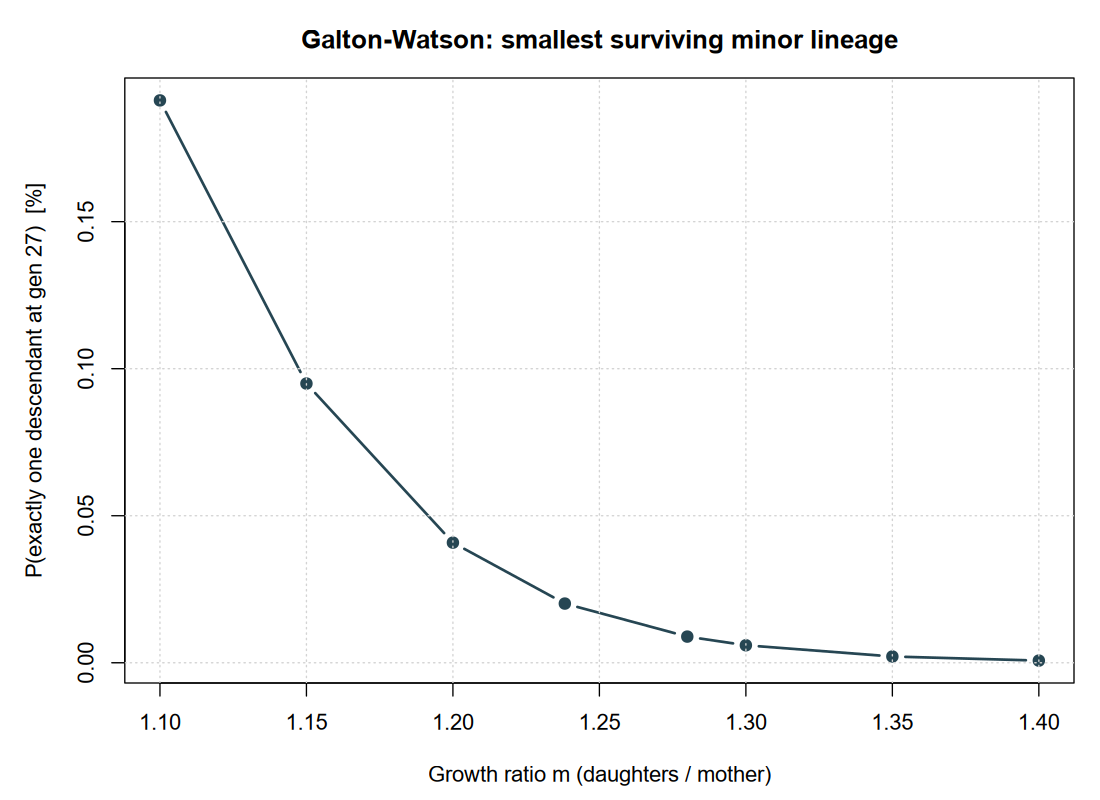
\includegraphics[width=0.82\linewidth]{../outputs/figures/A1_single_descendant.png}
\caption{Probability of a single surviving descendant at generation 27 versus growth ratio.}
\label{fig:a1}
\end{figure}
\begin{table}[htbp]
\centering
\small
\caption{Sensitivity of the branching model to the offspring law (Poisson vs. geometric).}
\label{tab:sens}
\begin{tabular}{lllll}
\toprule
Offspring model & Growth & P(extinct) & P(one) & P(>=3 desc) \\
\midrule
poisson &   1.1 & 0.8137 & 0.001912 & 0.1822 \\
poisson &  1.15 & 0.7476 & 0.0009495 & 0.2503 \\
poisson &   1.2 & 0.6852 & 0.0004085 & 0.3139 \\
poisson & 1.238 & 0.6412 & 0.0002013 & 0.3583 \\
poisson &  1.28 & 0.5968 & 0.00008896 & 0.403 \\
poisson &   1.3 & 0.5769 & 0.00005949 & 0.4229 \\
poisson &  1.35 & 0.5307 & 0.00002125 & 0.4693 \\
poisson &   1.4 & 0.489 & 0.000007408 & 0.511 \\
geometric &   1.1 & 0.9023 & 0.0007278 & 0.09623 \\
geometric &  1.15 & 0.8669 & 0.0004069 & 0.1323 \\
geometric &   1.2 & 0.8323 & 0.0002047 & 0.1673 \\
geometric & 1.238 & 0.8071 & 0.0001162 & 0.1926 \\
geometric &  1.28 & 0.781 & 0.00006111 & 0.2188 \\
geometric &   1.3 & 0.7691 & 0.00004471 & 0.2308 \\
geometric &  1.35 & 0.7407 & 0.00002035 & 0.2593 \\
geometric &   1.4 & 0.7143 & 0.000009257 & 0.2857 \\
\bottomrule
\end{tabular}
\end{table}
\begin{figure}[htbp]
\centering
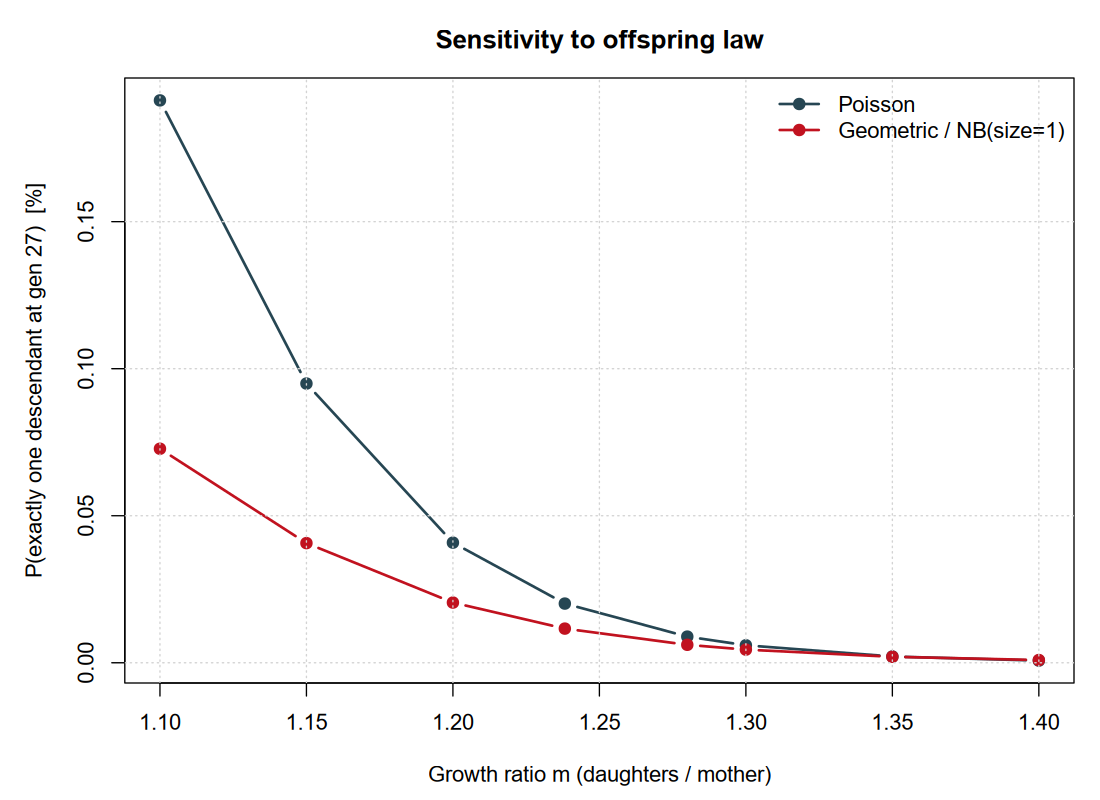
\includegraphics[width=0.82\linewidth]{../outputs/figures/A2b_offspring_law_sensitivity.png}
\caption{Single-descendant probability under Poisson and geometric (overdispersed) offspring laws.}
\label{fig:a2b}
\end{figure}
\begin{figure}[htbp]
\centering
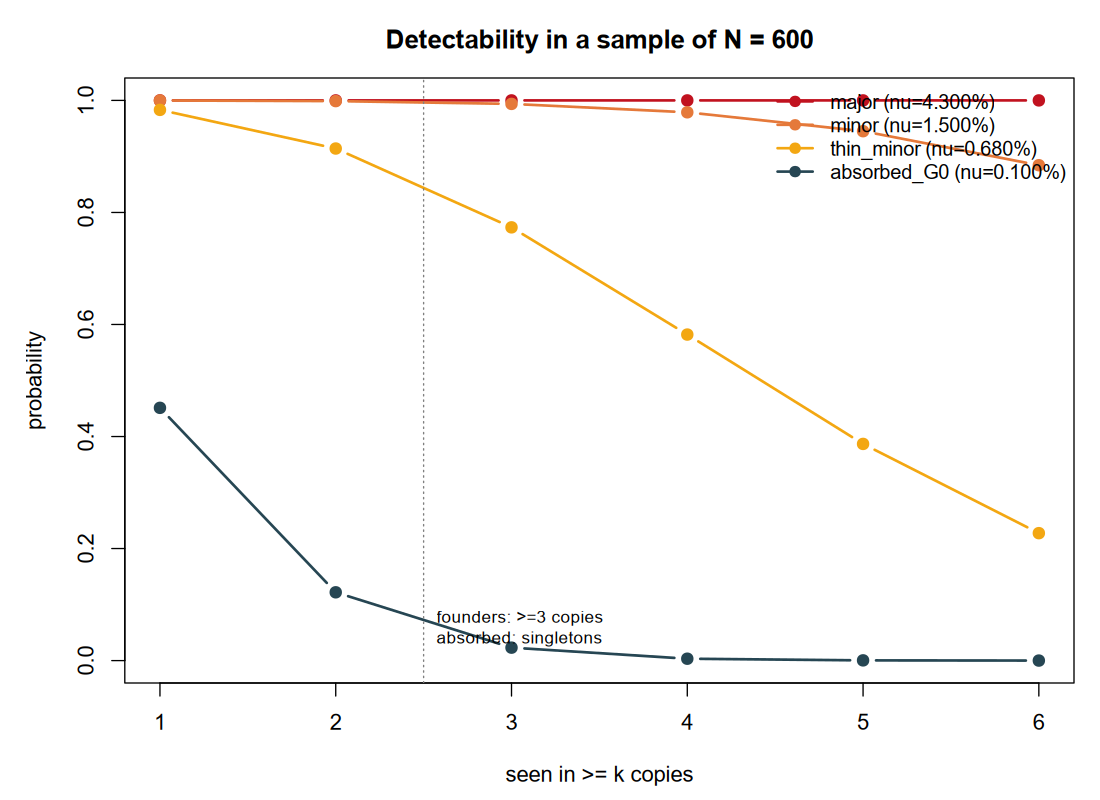
\includegraphics[width=0.82\linewidth]{../outputs/figures/A2_detection_curves.png}
\caption{Detectability of founder versus absorbed lineages in a sample of $N=600$ (cumulative Poisson).}
\label{fig:a2}
\end{figure}
\subsection{A simple extension: intermediate reproductive overdispersion}
The Poisson-versus-geometric contrast spans only the extremes of a single axis, reproductive overdispersion. A negative-binomial offspring law with dispersion $\phi$ has variance $m + m^2/\phi$, so $\phi=1$ is geometric and $\phi\to\infty$ is Poisson. Sweeping intermediate dispersions (Table~\ref{tab:nb}, Figure~\ref{fig:d1}) shows the single-descendant and extinction probabilities vary smoothly between the extremes: no member of this family removes the conclusion that exact single-descendant survival is a rare tail event.

\begin{table}[htbp]
\centering
\footnotesize
\caption{Single-descendant and extinction probabilities across the negative-binomial size ladder (geometric $=1$, Poisson $=\infty$), at three growth ratios.}
\label{tab:nb}
\begin{tabular}{lllll}
\toprule
Offspring law & Growth & Var/mean & P(extinct) & P(one desc) \\
\midrule
NB(size=0.5) &  1.15 &   3.3 & 0.9096 & 0.0002378 \\
NB(size=1) &  1.15 &  2.15 & 0.8669 & 0.0004077 \\
NB(size=2) &  1.15 & 1.575 & 0.8257 & 0.0005895 \\
NB(size=5) &  1.15 &  1.23 & 0.786 & 0.0007726 \\
NB(size=20) &  1.15 & 1.058 & 0.7584 & 0.0008999 \\
Poisson (size=Inf) &  1.15 &     1 & 0.7476 & 0.0009495 \\
NB(size=0.5) &   1.2 &   3.4 & 0.8858 & 0.0001244 \\
NB(size=1) &   1.2 &   2.2 & 0.8323 & 0.0002047 \\
NB(size=2) &   1.2 &   1.6 & 0.7811 & 0.0002819 \\
NB(size=5) &   1.2 &  1.24 & 0.7321 & 0.0003508 \\
NB(size=20) &   1.2 &  1.06 & 0.6984 & 0.0003932 \\
Poisson (size=Inf) &   1.2 &     1 & 0.6852 & 0.0004085 \\
NB(size=0.5) &  1.28 &  3.56 & 0.8499 & 0.00004091 \\
NB(size=1) &  1.28 &  2.28 & 0.781 & 0.00006111 \\
NB(size=2) &  1.28 &  1.64 & 0.716 & 0.00007617 \\
NB(size=5) &  1.28 & 1.256 & 0.6547 & 0.00008536 \\
NB(size=20) &  1.28 & 1.064 & 0.613 & 0.00008846 \\
Poisson (size=Inf) &  1.28 &     1 & 0.5968 & 0.00008896 \\
\bottomrule
\end{tabular}
\end{table}
\begin{figure}[htbp]
\centering
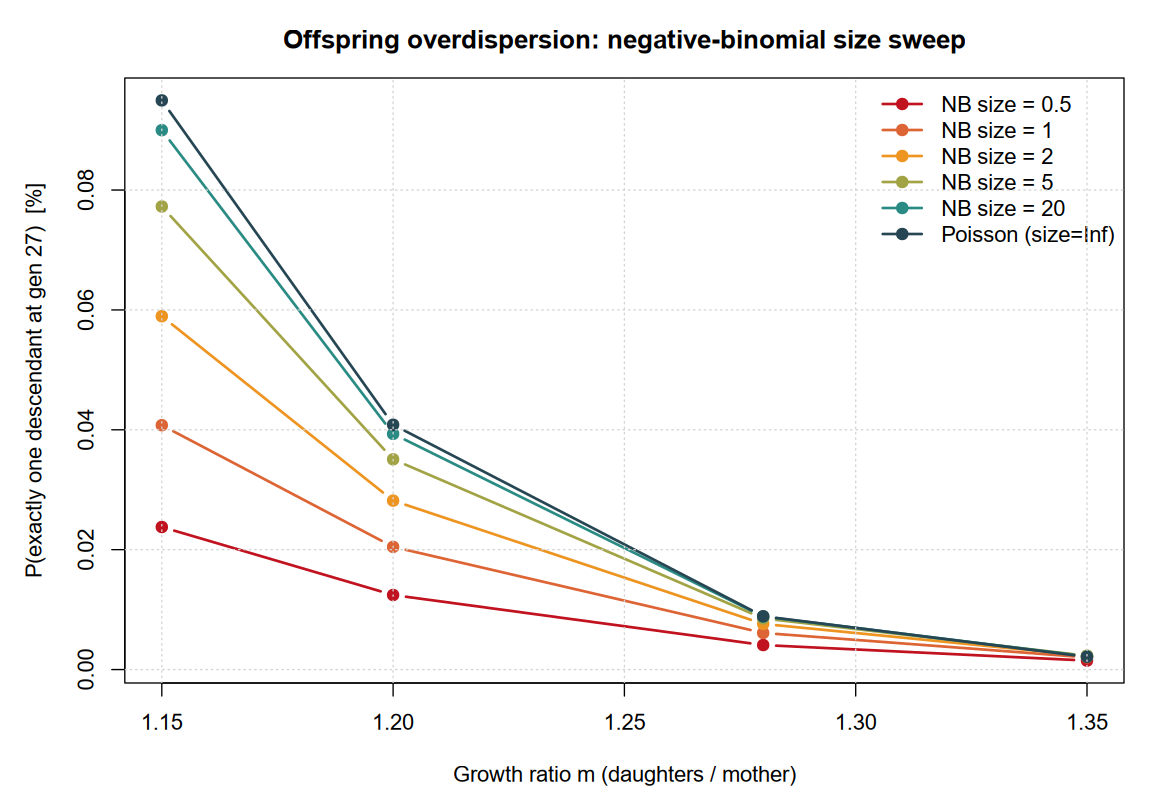
\includegraphics[width=0.82\linewidth]{../outputs/figures/D1_nbinom_size.png}
\caption{Single-descendant probability across the negative-binomial dispersion ladder.}
\label{fig:d1}
\end{figure}
\subsection{A complex extension: piecewise historical growth}
A single constant growth ratio is demographically unrealistic. We replace it with a piecewise per-generation schedule (Table~\ref{tab:sch}): a near-stationary medieval founder phase followed by rapid modern expansion, and compare it against a constant-growth process matched on \emph{net} expansion. Holding total growth fixed at about 320.0-fold over 27 generations, the realistic schedule raises extinction to 82.5\% (from 64.1\%) and lowers the singleton probability to 0.00\% (from 0.02\%; Figure~\ref{fig:d2}). Early stasis prunes more lineages while rapid late expansion leaves survivors in many copies, so realistic history sharpens rather than weakens the founder-versus-host distinction.

\begin{table}[htbp]
\centering
\small
\caption{Calendar-anchored piecewise growth schedule over 27 generations.}
\label{tab:sch}
\begin{tabular}{lll}
\toprule
Phase & Generations & Growth ratio \\
\midrule
medieval\_stasis & 1-7 & 1.001 \\
early\_modern & 8-17 & 1.361 \\
great\_expansion & 18-23 & 1.561 \\
modern & 24-27 & 1.001 \\
\bottomrule
\end{tabular}
\end{table}
\begin{figure}[htbp]
\centering
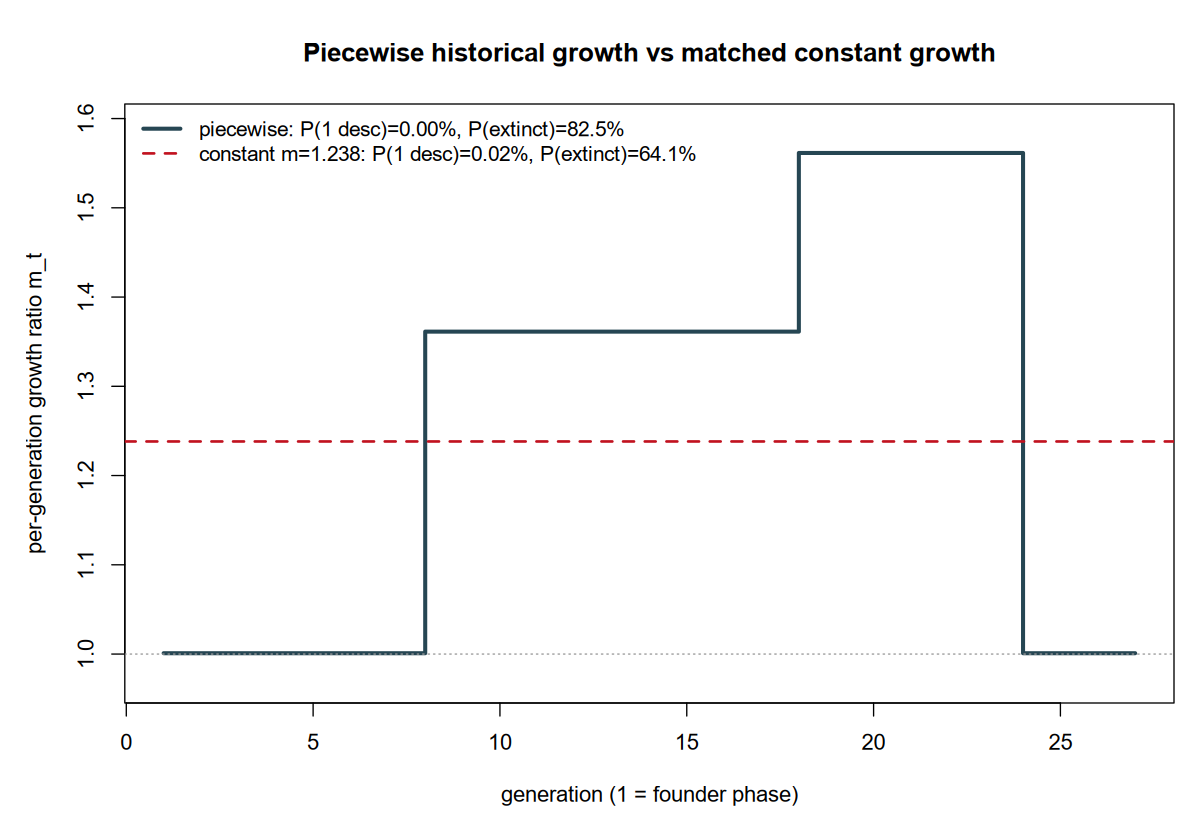
\includegraphics[width=0.82\linewidth]{../outputs/figures/D2_piecewise_growth.png}
\caption{Piecewise historical growth versus a constant-growth process matched on net expansion.}
\label{fig:d2}
\end{figure}
\subsection{A complex extension: origin synthesis (single fitted model)}
We combine the separate lines of evidence into a single posterior probability that each lineage is Near Eastern / Levantine (H2). Active inputs: Ashkenazi frequencies from Brook (2022) / Penninx (2019); non-Jewish frequencies from 1000 Genomes EUR (CEU+GBR+FIN+IBS+TSI, n=503) subclades with Mitotree fallback (Figure~\ref{fig:d3}). Three raw channels --- non-Jewish rarity, antiquity/time (depth, medieval carriers, public age), and equal-$n$ nesting --- are z-scored and combined by a ridge-logistic model fit to labeled controls with founders held out; the fitted channel weights are reported in Table~\ref{tab:fcoef} and the standardized founder channels in Table~\ref{tab:bscore}.

Leave-one-out validation on the 21 labeled lineages classifies \textbf{18 of 21 correctly (86\%)}, and the resulting per-founder posteriors are collected in Table~\ref{tab:bayes}.

\begin{table}[htbp]
\centering
\small
\caption{Fitted channel weights (posterior mean and 90 percent credible interval).}
\label{tab:fcoef}
\begin{tabular}{ll}
\toprule
Channel & Posterior weight \\
\midrule
Intercept & 0.55 [-0.71, 1.82] \\
Frequency (non-Jewish rarity) & 3.31 [1.29, 5.35] \\
Time (antiquity + carriers + public age) & 1.54 [0.15, 3.51] \\
Nesting (equal-n richness) & 1.17 [0.14, 2.48] \\
\bottomrule
\end{tabular}
\end{table}
\begin{table}[htbp]
\centering
\footnotesize
\caption{Standardized channel values for founders.}
\label{tab:bscore}
\begin{tabular}{llllll}
\toprule
Founder & z(freq) & z(time) & z(nest) & rarity & nest frac \\
\midrule
K1a1b1a & 0.5659 & 1.956 & 1.087 & 0.2104 & 0.06897 \\
K1a9 & 0.9208 & 1.859 & 1.087 & 0.6615 & 0.06897 \\
K2a2a & 0.6745 & -0.05464 & 0 & 0.3615 &    NA \\
N1b2 & 0.7916 & 0.2299 & -0.6449 & 0.5952 & -0.001596 \\
\bottomrule
\end{tabular}
\end{table}
\begin{table}[htbp]
\centering
\small
\caption{Posterior probability of a Near Eastern / Levantine origin (H2) per founder, with 90 percent credible intervals.}
\label{tab:bayes}
\begin{tabular}{lllll}
\toprule
Founder & Post mean & q05 & Median & q95 \\
\midrule
K1a1b1a & 0.9877 & 0.9413 & 0.9983 &     1 \\
K1a9 & 0.9939 & 0.9731 & 0.9994 &     1 \\
K2a2a & 0.899 & 0.6703 & 0.9367 & 0.9909 \\
N1b2 & 0.8913 & 0.6075 & 0.9408 & 0.994 \\
\bottomrule
\end{tabular}
\end{table}
\begin{figure}[htbp]
\centering
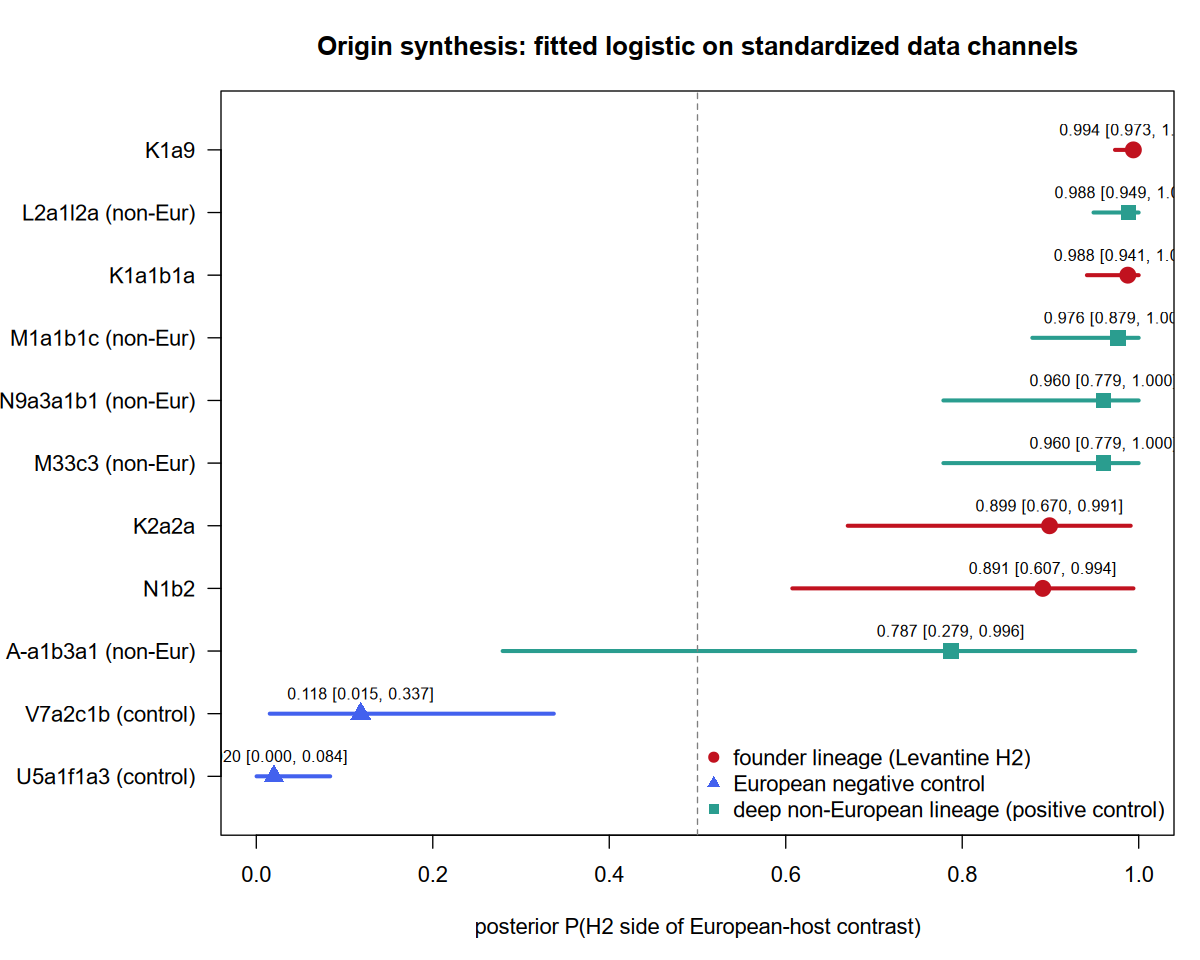
\includegraphics[width=0.82\linewidth]{../outputs/figures/D3_bayes_origin.png}
\caption{Origin synthesis: founders (red), European controls (blue), deep non-European controls (green); 90\% credible intervals from the fitted logistic on standardized data channels.}
\label{fig:d3}
\end{figure}
All four founders sit above 0.5: K1a1b1a 0.988, K1a9 0.994, K2a2a 0.899 and N1b2 0.891. N1b2's interval is the widest because the nesting channel is a negative contributor for it: at the N1b macro background its sister lineages remain Europe-richer at equal $n$, which tempers its positive rarity and time channels. K2a2a's sister pool in the Near East is a single sample once its own carriers are excluded, so its comparison climbs to K, where the sister richness is near parity; its score therefore rests mainly on rarity and antiquity. (We report three decimals because rounding would overstate certainty.)

\subsection{Negative controls: European (absorbed) Ashkenazi lineages}
A synthesis that returned a Levantine origin for \emph{every} Ashkenazi lineage would be uninformative, so we applied the identical model to a small manually parameterized calibration panel of lineages that are Ashkenazi-carried but European in phylogeographic origin, and required the model to place them well below 0.5. The inputs are literature-coded rather than estimated de novo from the Mitotree pipeline. The first, V7a2c1b, is not a rare oddity: it is a common, established Ashkenazi maternal cluster at about 2.4\% (Penninx, 2019; compiled in Brook, 2022; defining mutation A12753G), comparable to HV5a and not far below K2a2a. Its carriers include Yiddish-speaking individuals from Lithuania (YFull YF083232, YF108999), Galicia (GenBank OR803751, Dynow) and Ukraine (GenBank PQ337267, Berezna). Yet on every diagnostic that distinguishes origin it is the mirror image of the four founders: it nests inside an entirely European branch of haplogroup V (a post-glacial European expansion) rather than K1a/K2a/N1b; within the same subclade it is shared with non-Jewish Europeans (Danish KF162774, Russian JQ703830, and German and Belarusian samples), so the near-absence-among-non-Jews signal that flags the founders is absent; and it has no deep Near Eastern ancient record and no medieval Jewish (Erfurt/Tarrega) carrier.

We deliberately avoid a \emph{too-young} argument, because the age of this branch is uncertain: YFull dates the tight subclade to about 100 years, whereas FamilyTreeDNA's Discover tool (which names the same branch V7a12a1) suggests a TMRCA near 371 BCE (95\% CI 696--66 BCE; about 2,400 years). Coalescence age alone does not indicate a Near Eastern origin, and granting V7a2c1b even a Roman-era age does not move it toward H2, because its European signal comes entirely from nesting and non-Jewish sharing. V7a2c1b has only ten Near Eastern samples in its comparison pool even after the climb to HV0, sitting exactly on the minimum-pool floor and in the root with the largest naming-depth asymmetry in the panel, so we do not read its nesting value as evidence in either direction. The second control, U5a1f1a3, belongs to haplogroup U5 --- the signature European Mesolithic hunter-gatherer lineage, which dominates pre-Neolithic Europe and is essentially absent from the Pre-Pottery Neolithic Near East (Fernandez et al., 2014, recover K, not U5, in PPNB farmers). Any Ashkenazi U5 lineage is thus European by deep phylogeography, and because U5 is common in non-Jewish Europeans its non-Jewish-rarity signal is strongly negative. It provides an independent European control with a different origin story (Paleolithic hunter-gatherer versus post-glacial V), guarding against the objection that the V7a2c1b result is a one-off.

Under the same fitted synthesis, the two controls return $P(\text{H2}) = 0.12$ (90\% CI 0.02--0.34) for V7a2c1b and $0.02$ (0.00--0.08) for U5a1f1a3 --- far below all four founders (0.89--0.99; Table~\ref{tab:nc}, Figure~\ref{fig:d3}). 1000 Genomes EUR subclade frequencies (V 3.0\%, U5a1 4.2\%) supply the non-Jewish-rarity contrast that Table~7 alone cannot provide for non-founder lineages.

\begin{table}[htbp]
\centering
\footnotesize
\caption{Negative-control lineages: non-Jewish frequency, standardized channels, and posterior origin probability.}
\label{tab:nc}
\begin{tabular}{llllllll}
\toprule
Lineage & non-Jew freq & z(freq) & z(time) & z(nest) & Post mean & q05 & q95 \\
\midrule
U5a1f1a3 (control) & 0.04175 & -0.9208 & -1.164 & -0.6583 &  0.02 & 0.000343 & 0.08373 \\
V7a2c1b (control) & 0.02982 & -0.5659 & -0.6922 & 0 & 0.1184 & 0.01528 & 0.3371 \\
\bottomrule
\end{tabular}
\end{table}
The two negative controls are intentionally sparse but mechanistically different. V7a2c1b tests a common Ashkenazi cluster that is nevertheless shared with non-Jewish Europeans; U5a1f1a3 tests a deep European hunter-gatherer macro-clade. This guards against two failure modes: a classifier that simply rewards Ashkenazi frequency, and a classifier that cannot recognize older European lineages.

\subsection{Positive controls: deep non-European lineages through the same model}
The founders and the European host lineages are not the whole story. The Ashkenazi maternal pool also contains lineages whose \emph{deep} origin is neither European nor Levantine but African or Asian, and their presence is hard to reconcile with the strong form of H1 (recent assimilation from European hosts), because a European source cannot contribute African or East Asian mtDNA. The largest is L2a1l2a (about 2.2\% of Ashkenazi maternal lines; Penninx, 2019; Brook, 2022), a lineage of deep Sub-Saharan/East African origin already present in the 14th-century Erfurt Jewish cemetery (individual I13865). Several smaller lineages of African or Asian deep origin tell the same story.

We run these through the \emph{identical} synthesis as a manually parameterized positive-control panel, which is instructive once the axis is read correctly. The model contrasts a recent \emph{European-host} origin (H1) with a Near Eastern / Jewish-diaspora origin (H2); for the four founders the H2 pole is specifically Levantine, whereas for these lineages it means entry through the non-European diaspora rather than a literal Levantine birthplace. A high posterior is therefore a rejection of European-host assimilation. Because these clades are essentially absent among non-Jewish Europeans and nest entirely outside European diversity (with medieval Jewish carriers where documented), the model places them firmly on the non-European side (Table~\ref{tab:noneur}).

\begin{table}[htbp]
\centering
\footnotesize
\caption{Ashkenazi maternal lineages of deep African or Asian origin, scored under the identical synthesis (frequencies Penninx 2019 / Brook 2022; Erfurt from Waldman et al. 2022).}
\label{tab:noneur}
\begin{tabular}{lllll}
\toprule
Lineage & Deep origin & Ashk pct & Erfurt & Post P(H2-side) \\
\midrule
A-a1b3a1 & East Asian / Siberian (macrohaplogroup A) &  0.06 & -- & 0.79 \\
L2a1l2a & Sub-Saharan / East African (L2) &   2.2 & I13865 (Erfurt-ME) & 0.99 \\
M1a1b1c & North African / Near Eastern back-migration (M1) &  0.31 & -- & 0.98 \\
M33c3 & South Asian (M33) &  0.34 & -- & 0.96 \\
N9a3a1b1 & East Asian / Central Eurasian (N9a) &  0.52 & I14740 (Erfurt-EU) & 0.96 \\
\bottomrule
\end{tabular}
\end{table}
All five land above 0.5 (posterior means 0.79--0.99), \emph{with} the founders and opposite the European controls (Figure~\ref{fig:d3}); the two lineages with a documented Erfurt carrier (L2a1l2a and N9a3a1b1) are scored with that medieval Jewish anchor contributing to their time channel. This is exactly the intended discriminant behaviour: the same machinery scores genuinely European lineages low and genuinely non-European lineages high. Together these deep African/Asian lineages account for roughly 3.4\% of Ashkenazi maternal lines, and their complementary message is that the Ashkenazi maternal pool was assembled by a population that acquired lineages from Africa and Asia through the cosmopolitan diaspora history of a Near Eastern / Mediterranean Jewish community, not by recent absorption from northern-European hosts. For these lineages a high posterior means non-European, not specifically Levantine; their deep origin is African or Asian.

\subsection{Calibration on the broader frequent Ashkenazi pool}
The four founders account for a large minority, not the entirety, of the Ashkenazi maternal pool. To test whether the synthesis tracks the published literature in both directions, we scored a small literature-coded panel of frequent non-founder lineages spanning the origin spectrum with the same transformations and posterior (Table~\ref{tab:major}). This is a calibration analysis, not a new population-frequency estimate: a useful classifier should place lineages with published European assignments on the European side while retaining lineages with published Near Eastern assignments on the Near Eastern side, and should expose disputed cases rather than counting them as validation successes.

The Near Eastern side of this panel is deliberately conservative: Costa et al. (2013), despite arguing for substantial European maternal ancestry, classify HV1b2, R0a-associated lineages and U7 as Near Eastern sources and describe U1 as ultimately Near Eastern. Shamoon-Pour et al. (2019) further place HV1b2 near Assyrian HV1b branches in northern Mesopotamia and the South Caucasus, a plausible context for ancient Jewish communities. HV1b2 and U1b1a1 are also documented in the 14th-century Erfurt Jewish cemetery. Against these we set frequent lineages with published European assignments (H7 and J1c7a) and two deliberately ambiguous test cases, H6a1a1a and K1a4a. Brook/Wexler appear to treat the Ashkenazi H6a1a1a/H6a1a1a1 line as Middle Eastern, whereas the public Mitotree/FTDNA context and the supported parent H6a1a look Europe-rich. It is therefore not counted as a clean European validation control.

\begin{table}[htbp]
\centering
\footnotesize
\caption{Broader frequent Ashkenazi lineages scored under the identical synthesis, with published origin (Costa et al. 2013; Shamoon-Pour et al. 2019) and the model's call.}
\label{tab:major}
\begin{tabular}{lllll}
\toprule
Lineage & Ashk pct & Published & Post P(H2) & Model call \\
\midrule
H1 &     3 & European & 0.07 & European \\
H3 &   1.5 & European & 0.08 & European \\
H5 &   1.5 & European & 0.12 & European \\
H6a1a1a &  0.57 & Ambiguous & 0.58 & Near Eastern \\
H7 &   1.9 & European & 0.18 & European \\
HV1a &   1.5 & Near Eastern & 0.75 & Near Eastern \\
HV1b2 &  3.99 & Near Eastern & 0.86 & Near Eastern \\
I &   1.3 & European & 0.42 & European \\
J1c7a &   2.3 & European & 0.04 & European \\
K1a4a &   0.2 & Ambiguous & 0.29 & European \\
R0a &  2.52 & Near Eastern & 0.89 & Near Eastern \\
T2 &   4.8 & European & 0.05 & European \\
U1b1a1 &   0.8 & Near Eastern & 0.54 & Near Eastern \\
U4 &     1 & European & 0.12 & European \\
U7a5 &  1.55 & Near Eastern & 0.75 & Near Eastern \\
W &   1.6 & European & 0.29 & European \\
\bottomrule
\end{tabular}
\end{table}
The model agrees with the published origin in \textbf{14 of 14 evaluable} panel cases (Figure~\ref{fig:d4}); H6a1a1a, K1a4a are retained separately as ambiguous/disputed. The Near Eastern members all score high (0.54--0.89), whereas the clean European members (H1, H3, H5, H7, I, J1c7a, T2, U4, W) score low (0.04--0.42). The ambiguous H6a1a1a case also scores low (0.58), which is useful as a data-driven disagreement with a possible Brook Middle Eastern coding rather than as a validation point. This matters for interpretation in two ways. First, the four founders are not an isolated signal; several additional frequent Ashkenazi lineages, totaling roughly 10.4\% in the Brook/Penninx frequency compilation, are also Near Eastern under published phylogeographic assignments. Second, the low posteriors for the clean European controls show that the classifier is not biased toward H2: it reproduces European calls when the input evidence points that way, while exposing ambiguous cases.

\begin{figure}[htbp]
\centering
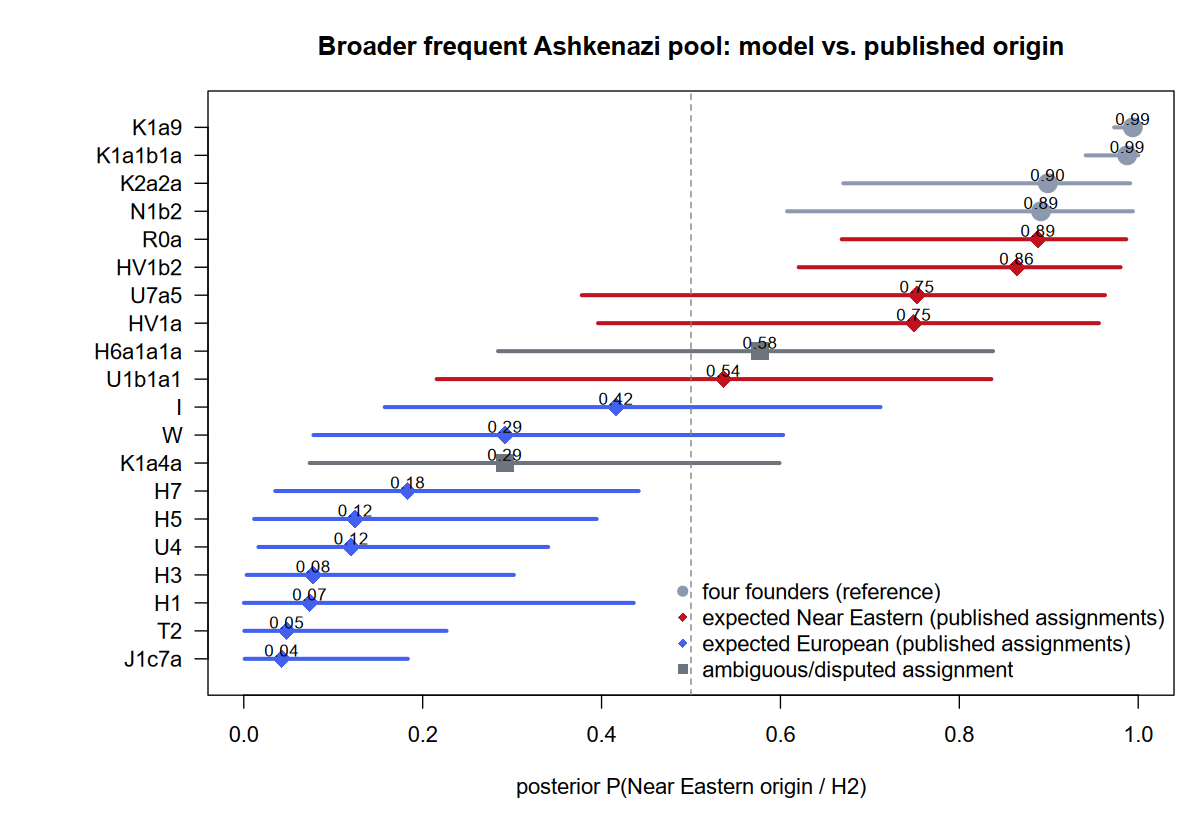
\includegraphics[width=0.82\linewidth]{../outputs/figures/D4_broader_pool.png}
\caption{Broader frequent Ashkenazi pool versus published origin: four founders (grey), lineages with published Near Eastern assignments (red diamonds), lineages with published European assignments (blue diamonds), and ambiguous/disputed lineages (grey squares).}
\label{fig:d4}
\end{figure}
\subsection{Founder clades are present and rare in the reference set}
All four founder clades are present in the enriched dataset and remain rare among modern reference samples (Table~\ref{tab:mt}, Figure~\ref{fig:a3}). K1a1b1a is the most frequent of the four and is anchored by 8 ancient/historical records, including medieval Jewish individuals. We interpret modern frequencies as rarity/context only, because modern country reflects diaspora residence rather than lineage origin.

\begin{table}[htbp]
\centering
\small
\caption{Founder-clade counts in the enriched, deduplicated reference set.}
\label{tab:mt}
\begin{tabular}{llllll}
\toprule
Founder & Modern n & Modern freq & Ancient n & Distinct hg & Known country \\
\midrule
K1a1b1a &    76 & 0.001321 &     8 &    21 &    31 \\
K1a9 &    26 & 0.0004519 &     1 &     8 &     5 \\
K2a2a &    39 & 0.0006779 &     3 &    12 &    26 \\
N1b2 &     8 & 0.0001391 & 0 &     3 &     3 \\
\bottomrule
\end{tabular}
\end{table}
\begin{figure}[htbp]
\centering
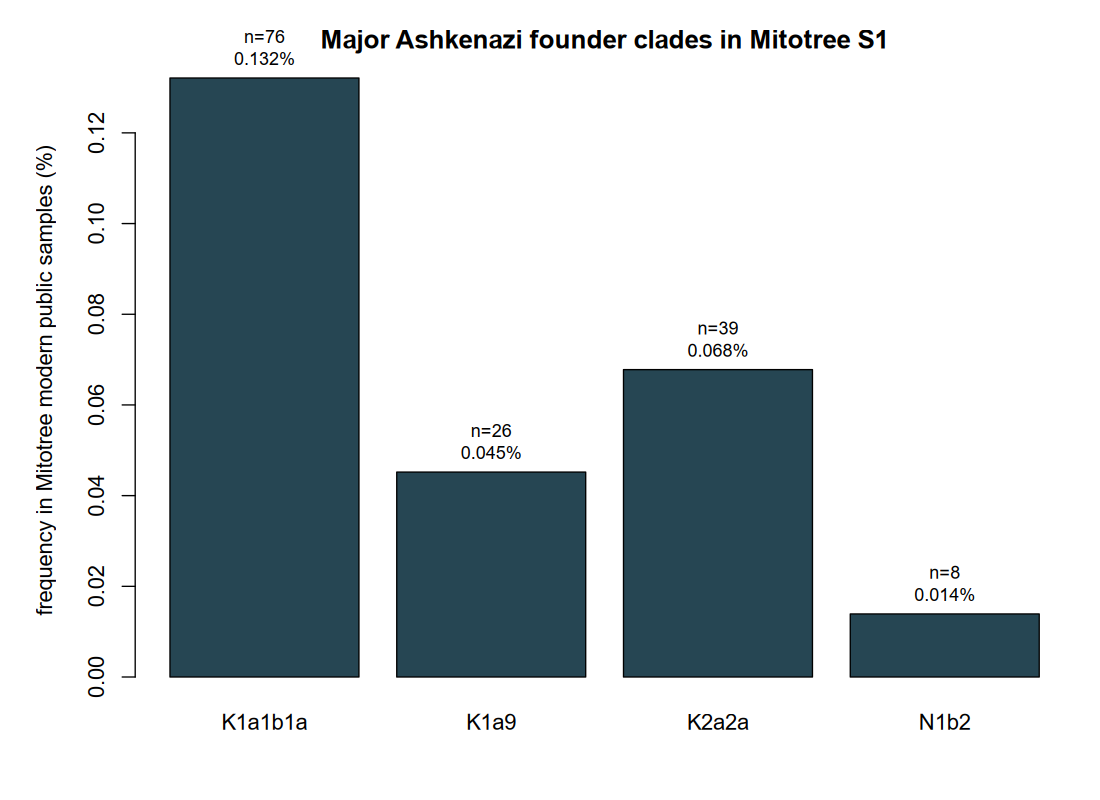
\includegraphics[width=0.82\linewidth]{../outputs/figures/A3_mitotree_founder_frequencies.png}
\caption{Frequency of the four major founder clades among modern Mitotree reference samples.}
\label{fig:a3}
\end{figure}
\subsection{Estimated host-lineage absorption rate}
Treating the enriched Mitotree+GenBank set as the largest available maternal sample, the individual-level singleton fraction is $a_\epsilon \approx 0.22$ (57,531 individuals), giving a per-generation absorption rate of roughly 0.76\%--0.97\% across founder-event depths $K = 25$--$32$ (Table~\ref{tab:abs}, Figure~\ref{fig:a4}). The dedicated Behar 2006 Ashkenazi sample yields a lower absorbed fraction ($\approx 0.13$) and rate, as expected: the enriched set is global, only a small fraction is explicitly Ashkenazi, and it over-counts rare non-founder lineages. Its singleton fraction is, however, strongly a function of how many samples were drawn and how finely the tree labels them rather than of absorption: rarefying the same pool gives $a_\epsilon$ from 0.22 at $n = 57{,}531$ to 0.96 at $n = 100$, and truncating the clade label from full depth to one character takes it from 0.22 to 0.00 (Table~\ref{tab:absid}). The enriched set's LOW value therefore reflects its large $n$, not less absorption, and the two estimates are comparable only at equal $n$ and equal clade resolution. We report both with Behar as the population-appropriate anchor. Under either estimate the four major founders lie far out in the multi-copy tail rather than among the absorbed singletons.

\begin{table}[htbp]
\centering
\footnotesize
\caption{Estimated host-lineage absorption from the largest available sample and the Behar 2006 benchmark.}
\label{tab:abs}
\begin{tabular}{llllll}
\toprule
Sample & n & a\_eps & K & Rate/gen & Absorbed surviving \\
\midrule
enriched\_mitotree\_modern & 57531 & 0.2172 &    25 & 0.00975 & 467.7 \\
enriched\_mitotree\_modern & 57531 & 0.2172 &    27 & 0.00903 & 665.1 \\
enriched\_mitotree\_modern & 57531 & 0.2172 &    32 & 0.00762 &  1636 \\
jewish\_flagged\_modern &   187 & 0.7273 &    25 & 0.05064 &  2430 \\
jewish\_flagged\_modern &   187 & 0.7273 &    27 & 0.04698 &  3461 \\
jewish\_flagged\_modern &   187 & 0.7273 &    32 & 0.03979 &  8542 \\
behar2006\_ashkenazi &   565 & 0.1257 &    25 & 0.00536 & 257.1 \\
behar2006\_ashkenazi &   565 & 0.1257 &    27 & 0.00496 & 365.5 \\
behar2006\_ashkenazi &   565 & 0.1257 &    32 & 0.00419 & 899.1 \\
\bottomrule
\end{tabular}
\end{table}
\begin{table}[htbp]
\centering
\footnotesize
\caption{Identifiability of the absorbed-fraction estimate: the singleton fraction of one unchanging pool, varied only by sample size and by clade-label depth.}
\label{tab:absid}
\begin{tabular}{llllll}
\toprule
Varied & Setting & n & Resolution & a\_eps & Rate/gen \\
\midrule
sample\_size & 100 &   100 & full & 0.9585 & 0.1112 \\
sample\_size & 565 &   565 & full & 0.9045 & 0.08332 \\
sample\_size & 2000 &  2000 & full & 0.8011 & 0.05805 \\
sample\_size & 10000 & 10000 & full & 0.5679 & 0.0306 \\
sample\_size & 57531 & 57531 & full & 0.2172 & 0.00903 \\
clade\_resolution & 1\_chars & 57531 & 1 chars & 0 & 0 \\
clade\_resolution & 3\_chars & 57531 & 3 chars & 0.0031 & 0.00011 \\
clade\_resolution & 4\_chars & 57531 & 4 chars & 0.0251 & 0.00094 \\
clade\_resolution & 6\_chars & 57531 & 6 chars & 0.1228 & 0.00484 \\
\bottomrule
\end{tabular}
\end{table}
\begin{figure}[htbp]
\centering
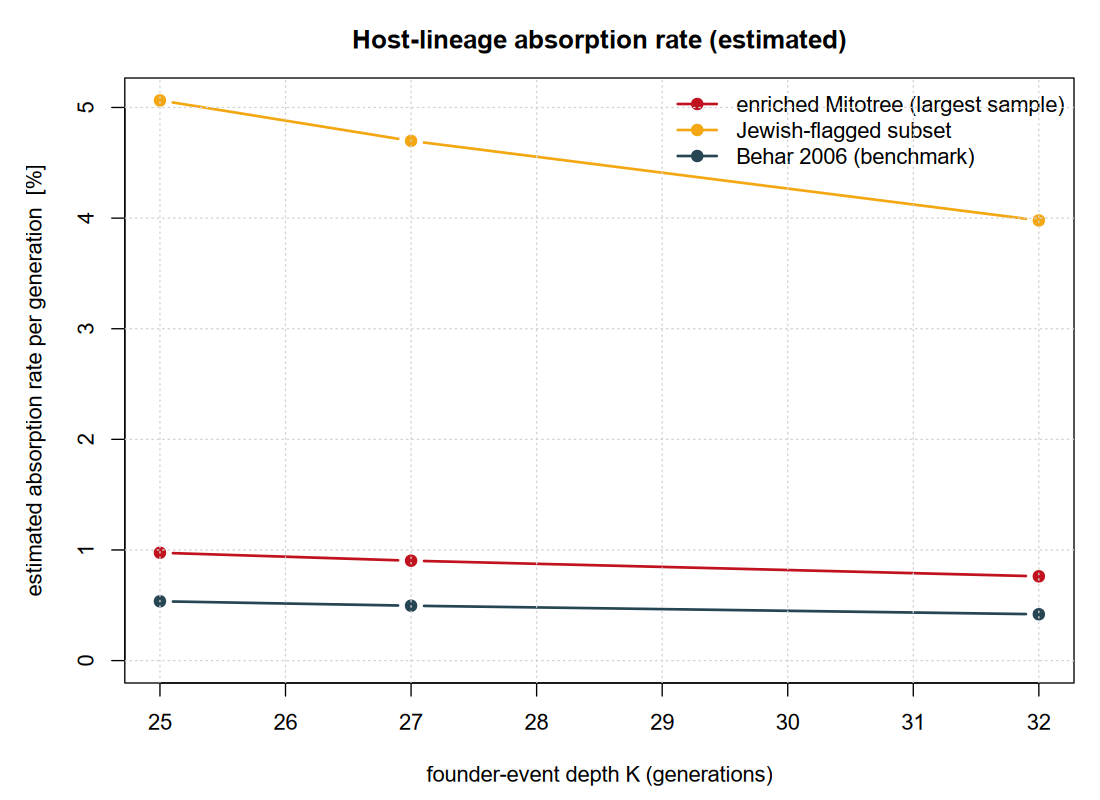
\includegraphics[width=0.82\linewidth]{../outputs/figures/A4_absorption_rate.png}
\caption{Estimated per-generation absorption rate versus founder-event depth.}
\label{fig:a4}
\end{figure}
Under the Livni--Skorecki 'Euro-Levantine' reconciliation scenario, a large Roman-era Jewish population produces three or more of the four major founders with probability 1.51\% at our base assumptions (Figure~\ref{fig:a6}). The per-lineage major-emergence probability, the private-mutation rate and the number of founder families are explicit assumptions rather than fitted quantities; varying each across a plausible range keeps this probability between 0.07\% and 24.26\% (Table~\ref{tab:elsens}), so the model-disfavored conclusion does not rest on any single value. We report this as a model sensitivity result, not as an empirical measurement.

\begin{figure}[htbp]
\centering
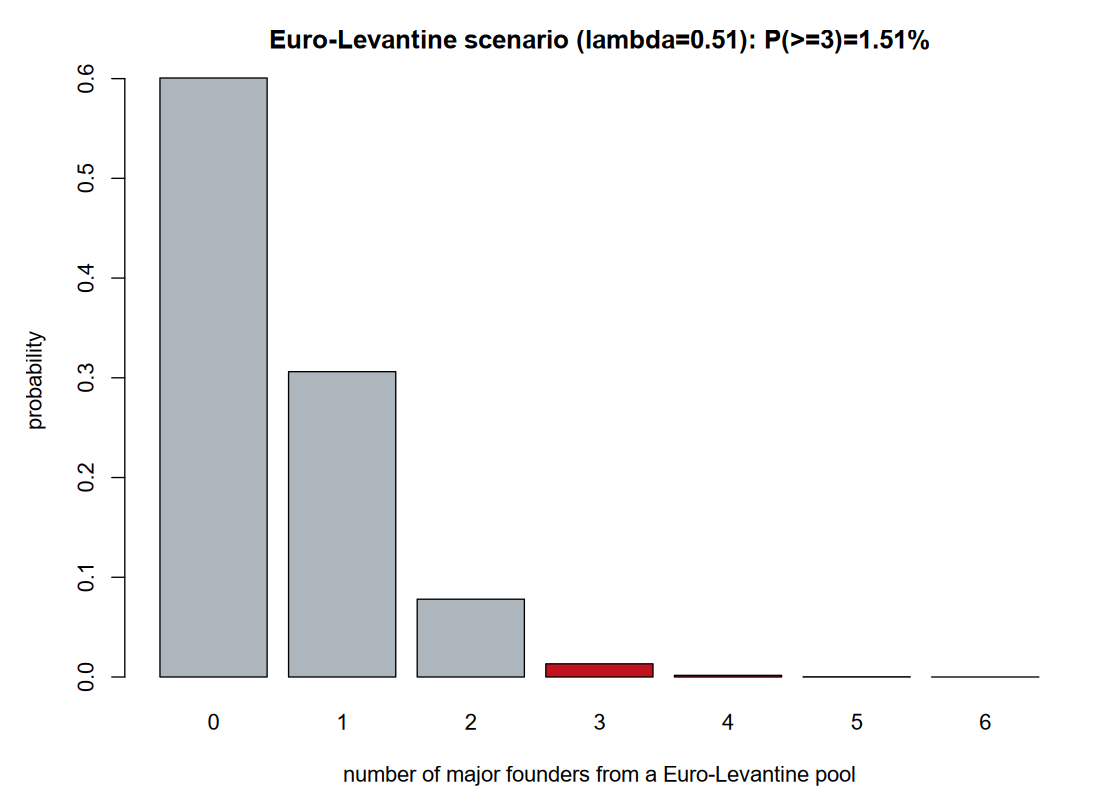
\includegraphics[width=0.82\linewidth]{../outputs/figures/A6_euro_levantine.png}
\caption{Probability of $\geq 3$ major founders arising in a large Euro-Levantine pool.}
\label{fig:a6}
\end{figure}
\begin{table}[htbp]
\centering
\footnotesize
\caption{Sensitivity of the Euro-Levantine feasibility to its three explicit assumptions (per-lineage major-emergence probability, private-mutation rate, founder families). P values are percentages.}
\label{tab:elsens}
\begin{tabular}{llllll}
\toprule
Assumption varied & Value & lambda & P(>=2) \% & P(>=3) \% & prob\_ge3\_major\_dirichlet\_sigma \\
\midrule
sigma\_major &  0.01 & 0.1699 &  1.29 & 0.072 & 0.05295 \\
sigma\_major &  0.02 & 0.3399 & 4.619 & 0.508 & 0.05295 \\
sigma\_major &  0.03 & 0.5098 & 9.318 & 1.514 & 0.05295 \\
sigma\_major & 0.049 & 0.8326 &  20.3 & 5.223 & 0.05295 \\
sigma\_major &  0.06 &  1.02 & 27.14 & 8.393 & 0.05295 \\
sigma\_major &   0.1 & 1.699 & 50.65 & 24.26 & 0.05295 \\
mu\_hv & 0.0029 & 0.4929 & 8.805 & 1.385 & 0.04882 \\
mu\_hv & 0.003006 & 0.5098 & 9.318 & 1.514 & 0.05295 \\
mu\_hv & 0.0043 & 0.7111 & 15.97 & 3.551 & 0.1137 \\
mu\_hv & 0.006 & 0.9602 & 24.96 & 7.312 & 0.2108 \\
founder\_families &   100 & 0.3399 & 4.619 & 0.508 & 0.1995 \\
founder\_families &   150 & 0.5098 & 9.318 & 1.514 & 0.05295 \\
founder\_families &   250 & 0.8496 & 20.91 & 5.482 & 0.0009206 \\
founder\_families &   350 &  1.19 & 33.36 & 11.82 & 0.000006593 \\
r &  0.03 & 0.5098 & 9.318 & 1.514 & 0.05295 \\
r &  0.05 & 0.5098 & 9.318 & 1.514 & 0.05295 \\
r &  0.07 & 0.5098 & 9.318 & 1.514 & 0.05295 \\
gens &    30 & 0.388 & 5.837 &  0.73 & 0.02697 \\
gens &    40 & 0.5098 & 9.318 & 1.514 & 0.05295 \\
gens &    50 & 0.6279 & 13.12 & 2.596 & 0.08619 \\
\bottomrule
\end{tabular}
\end{table}
\subsection{The 'solely European nesting' argument weakens after sampling control}
The Costa argument rests on counting more European than Near Eastern sub-lineages, but that count is confounded: the European reference sample is several-fold larger. When Europe and the Near East are rarefied to a common sample size the argument's premise weakens sharply (Figure~\ref{fig:b6}). For K1a, which contains K1a1b1a, sub-lineage richness is in fact higher in the Near East at equal sampling; for K2a and N1b it remains higher in Europe, so the nesting evidence ranges from positively Near Eastern (K1a) to inconclusive (K2a, N1b) but in no case supports the strong European-nesting claim once sampling is controlled. As a calibration check, the same rarefaction line-chart method was applied to literature-coded control clades in a separate companion panel: European-assigned controls (H, U5, J1c) are Europe-equal or Europe-richer, whereas Near Eastern-assigned controls (R0a, U7, U1) are Near-East-richer (Figure~\ref{fig:b6b}). The overall regional composition of the founder parent clades among reference samples with known country is shown in Figure~\ref{fig:b1}, and the immediate sibling clades of the founders are likewise not uniformly European (Figure~\ref{fig:b2}).

\begin{figure}[htbp]
\centering
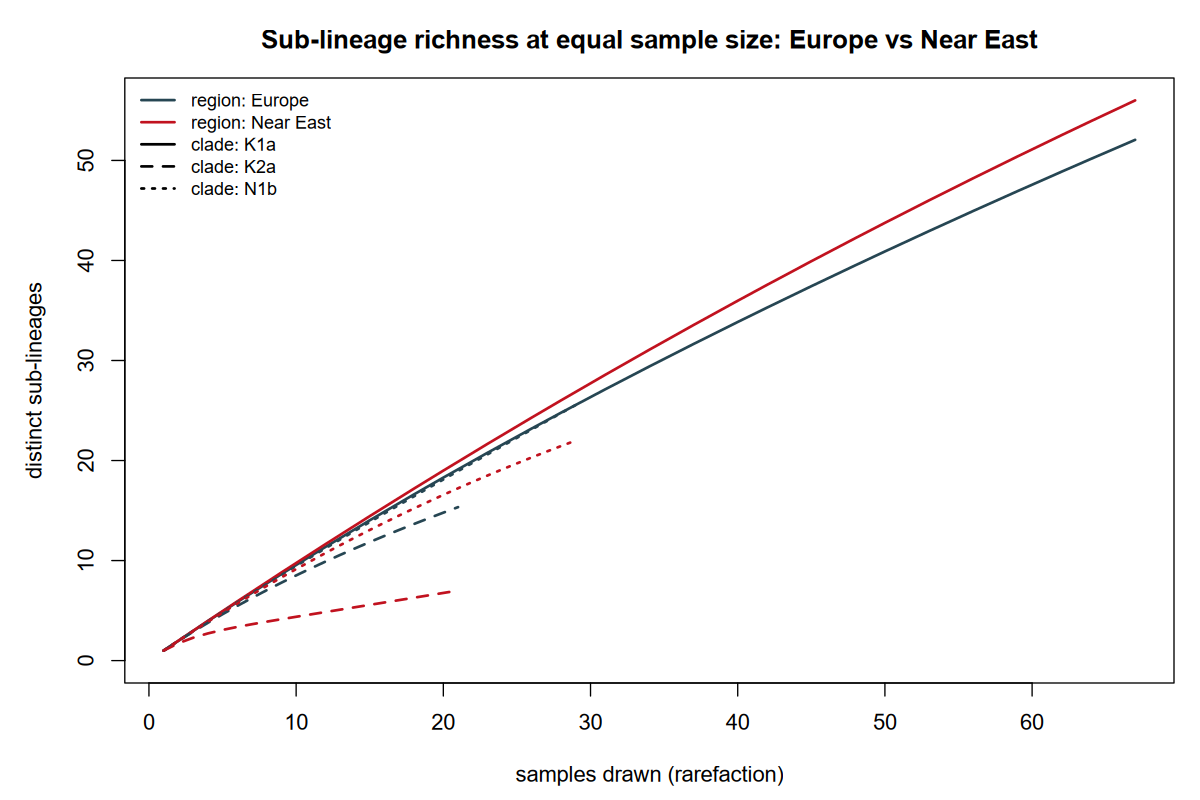
\includegraphics[width=0.82\linewidth]{../outputs/figures/B6_rarefaction.png}
\caption{Sub-lineage richness at equal sample size, Europe versus Near East.}
\label{fig:b6}
\end{figure}
\begin{figure}[htbp]
\centering
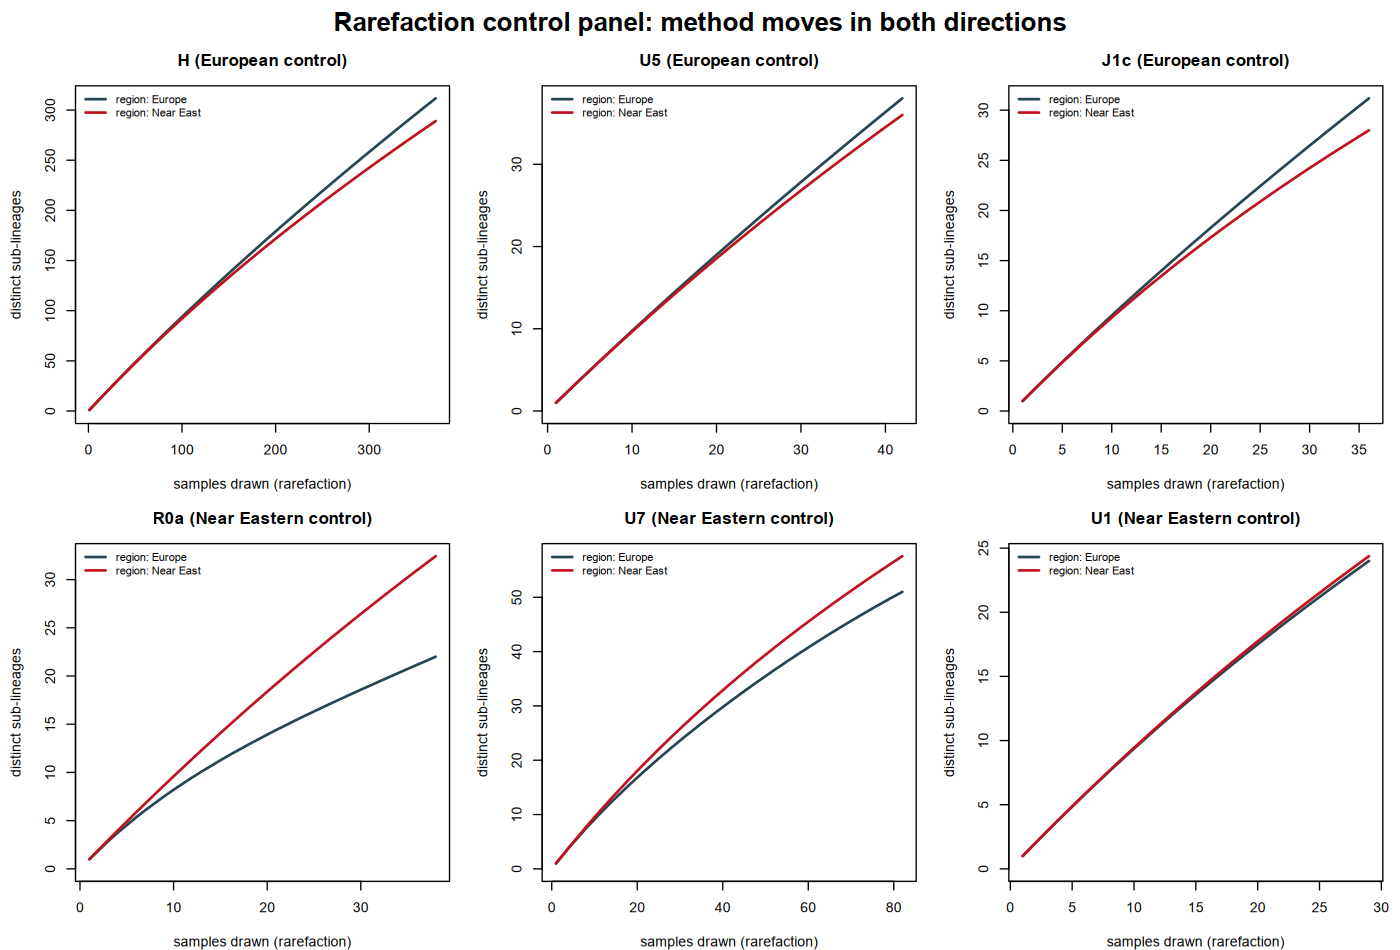
\includegraphics[width=0.82\linewidth]{../outputs/figures/B6b_rarefaction_controls.png}
\caption{Rarefaction control panel: European-assigned controls (H, U5, J1c) and Near Eastern-assigned controls (R0a, U7, U1), each plotted as Europe versus Near East at equal sample size. The companion panel shows the method can move in both directions and is not mechanically biased toward a Near Eastern result.}
\label{fig:b6b}
\end{figure}
\begin{figure}[htbp]
\centering
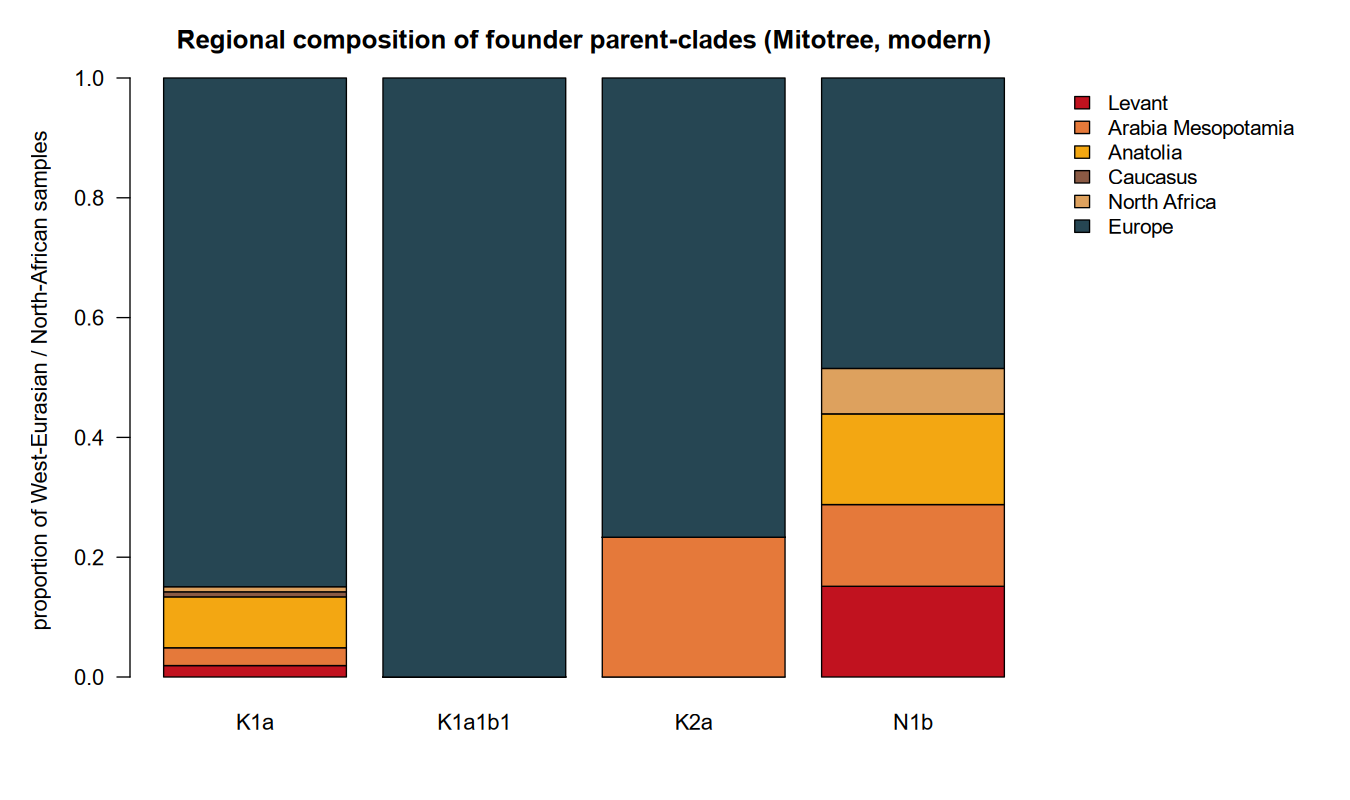
\includegraphics[width=0.82\linewidth]{../outputs/figures/B1_parentclade_region_props.png}
\caption{Regional composition of the parent clades (modern samples with known country).}
\label{fig:b1}
\end{figure}
\begin{figure}[htbp]
\centering
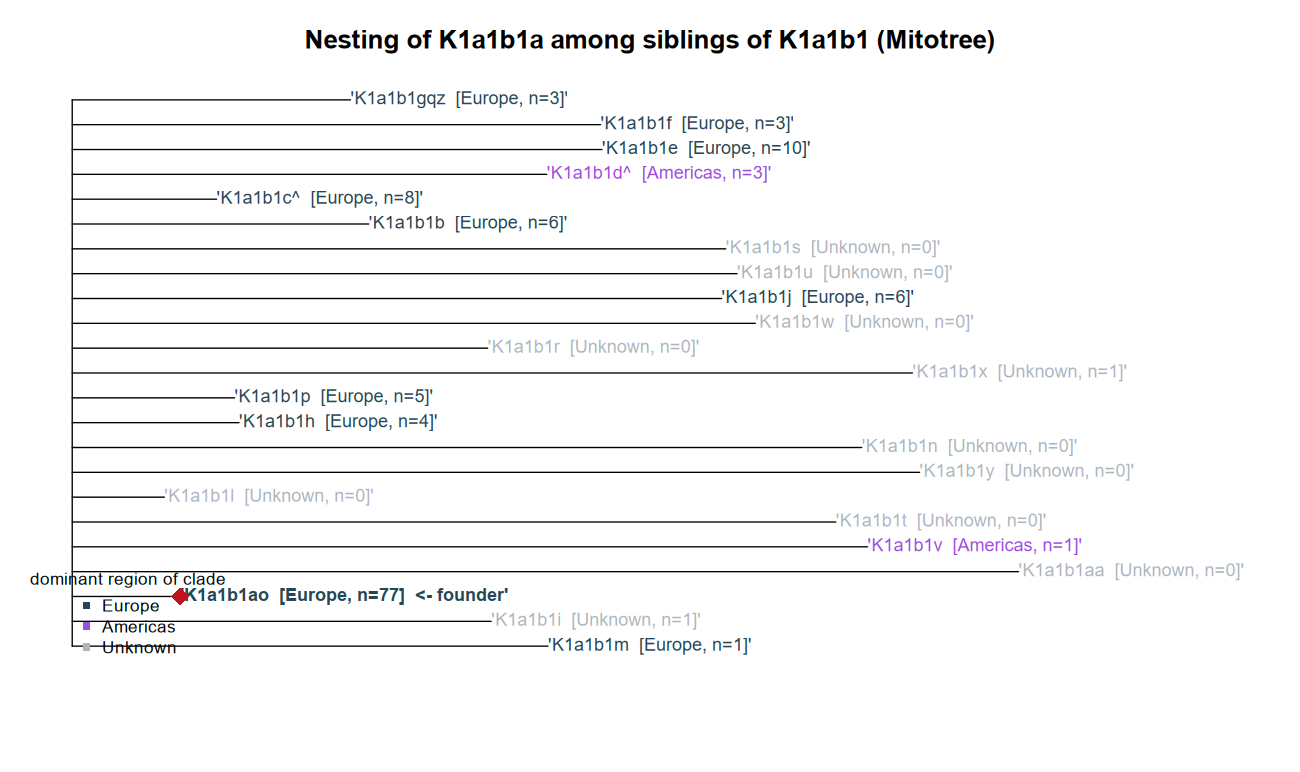
\includegraphics[width=0.82\linewidth]{../outputs/figures/B2_nesting_K1a1b1a.png}
\caption{K1a1b1a among the sibling clades of K1a1b1.}
\label{fig:b2}
\end{figure}
Decisively, the four founders are essentially absent among 27,651 non-Jews in the Livni--Skorecki / FTDNA benchmark (Table~\ref{tab:t7}, Figure~\ref{fig:b7}), with frequencies of order $10^{-4}$. If these lineages had entered the Ashkenazi gene pool by recent assimilation of local European women, they should be detectable at appreciable frequency in the surrounding non-Jewish populations; their near-absence is the single hardest observation for H1 to accommodate and is naturally explained if the founders entered with a Near Eastern source population. A reconstructed haplotype network of the founders together with their parent clades is shown in Figure~\ref{fig:b8}.

\begin{table}[htbp]
\centering
\small
\caption{Frequency of the four major founders among 27,651 non-Jews (Livni--Skorecki Table 7 reference benchmark).}
\label{tab:t7}
\begin{tabular}{llll}
\toprule
Haplotype & Count & Frequency & n non-Jews \\
\midrule
K1a9 &     6 & 0.000217 & 27651 \\
K1a1b1a &    17 & 0.000615 & 27651 \\
K2a2a &    12 & 0.000434 & 27651 \\
N1b2 &     7 & 0.000253 & 27651 \\
\bottomrule
\end{tabular}
\end{table}
\begin{figure}[htbp]
\centering
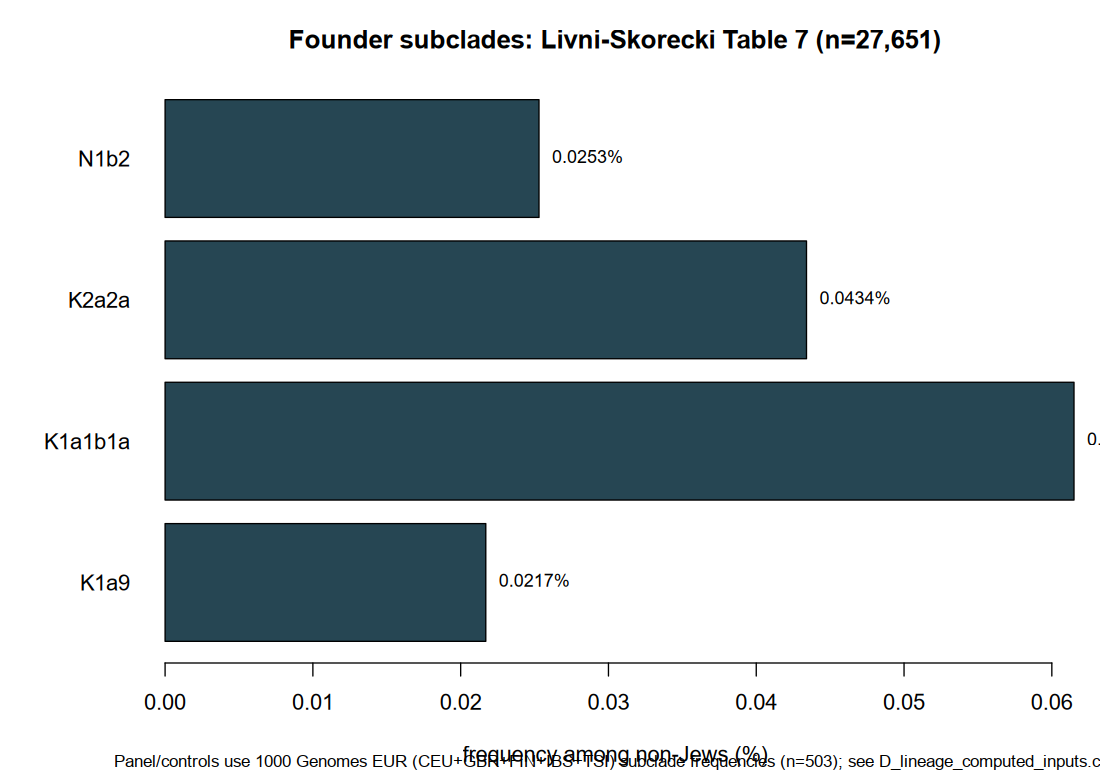
\includegraphics[width=0.82\linewidth]{../outputs/figures/B7_nonjewish_rarity.png}
\caption{Frequency of the four major founders among non-Jews.}
\label{fig:b7}
\end{figure}
\begin{figure}[htbp]
\centering
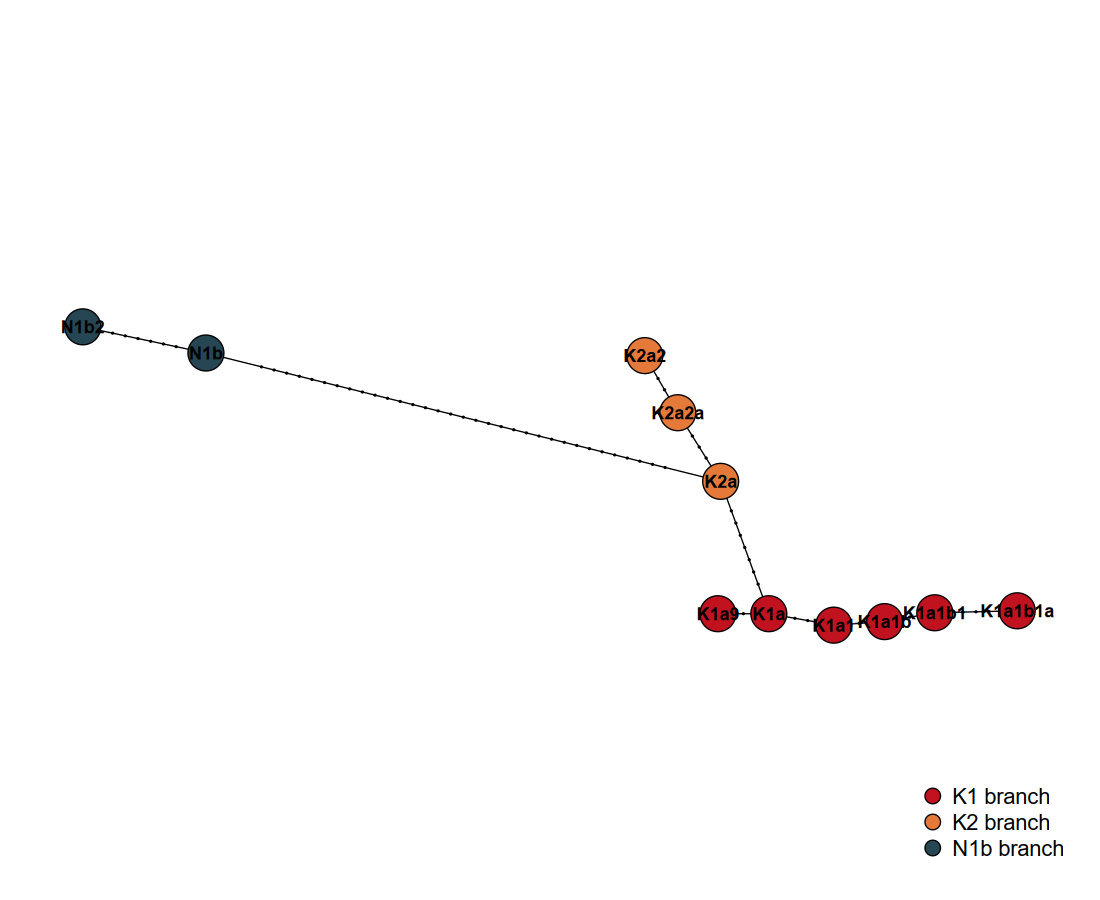
\includegraphics[width=0.82\linewidth]{../outputs/figures/B8_founder_haplonet.png}
\caption{Reconstructed haplotype network of the founders and their parent clades.}
\label{fig:b8}
\end{figure}
\subsection{Ancient DNA places the parent macro-clades deep in the Near East}
The oldest ancient K1a lineages in the enriched dataset are Near Eastern (Anatolia and the Levant), millennia before any Ashkenazi founder event (Table~\ref{tab:ne}, Figure~\ref{fig:c1}). Independently, Fernandez et al. (2014) report that haplogroup K is the most frequent lineage among Pre-Pottery Neolithic B farmers of Syria (K in 6 of 15 HVR1-typed individuals, about 40\%, in the profiles compiled here; Table~\ref{tab:ppnb}), with rare N* also present. These data are HVR1-level and therefore support the Near Eastern context of the K/N macro-clades rather than the derived Ashkenazi founder motifs themselves; nonetheless, they are difficult to reconcile with a purely European macro-clade narrative. The founders coalesce recently relative to their parent clades (Table~\ref{tab:coal}, Figure~\ref{fig:c2}), the expected signature of founder lineages.

\begin{table}[htbp]
\centering
\small
\caption{Oldest Near Eastern K1a records in the enriched dataset.}
\label{tab:ne}
\begin{tabular}{lllll}
\toprule
super\_clade & haplogroup & country & region & year \\
\midrule
K1a & K1a23c & Turkey & Anatolia & -8750 \\
K1a & K1a18b & Jordan & Levant & -8100 \\
K1a & K1a4 & Turkey & Anatolia & -6600 \\
K1a & K1a4 & Turkey & Anatolia & -6600 \\
K1a & K1a7d & Turkey & Anatolia & -6600 \\
K1a & K1a4 & Turkey & Anatolia & -6600 \\
K1a & K1a7d & Turkey & Anatolia & -6600 \\
K1a & K1a18c\char94{} & Turkey & Anatolia & -6525 \\
\bottomrule
\end{tabular}
\end{table}
\begin{table}[htbp]
\centering
\small
\caption{PPNB Near Eastern Neolithic haplogroup composition (Fernandez et al. 2014).}
\label{tab:ppnb}
\begin{tabular}{ll}
\toprule
Haplogroup & Count \\
\midrule
K &     6 \\
R0 &     3 \\
H &     2 \\
HV &     1 \\
L3 &     1 \\
N* &     1 \\
U* &     1 \\
\bottomrule
\end{tabular}
\end{table}
\begin{figure}[htbp]
\centering
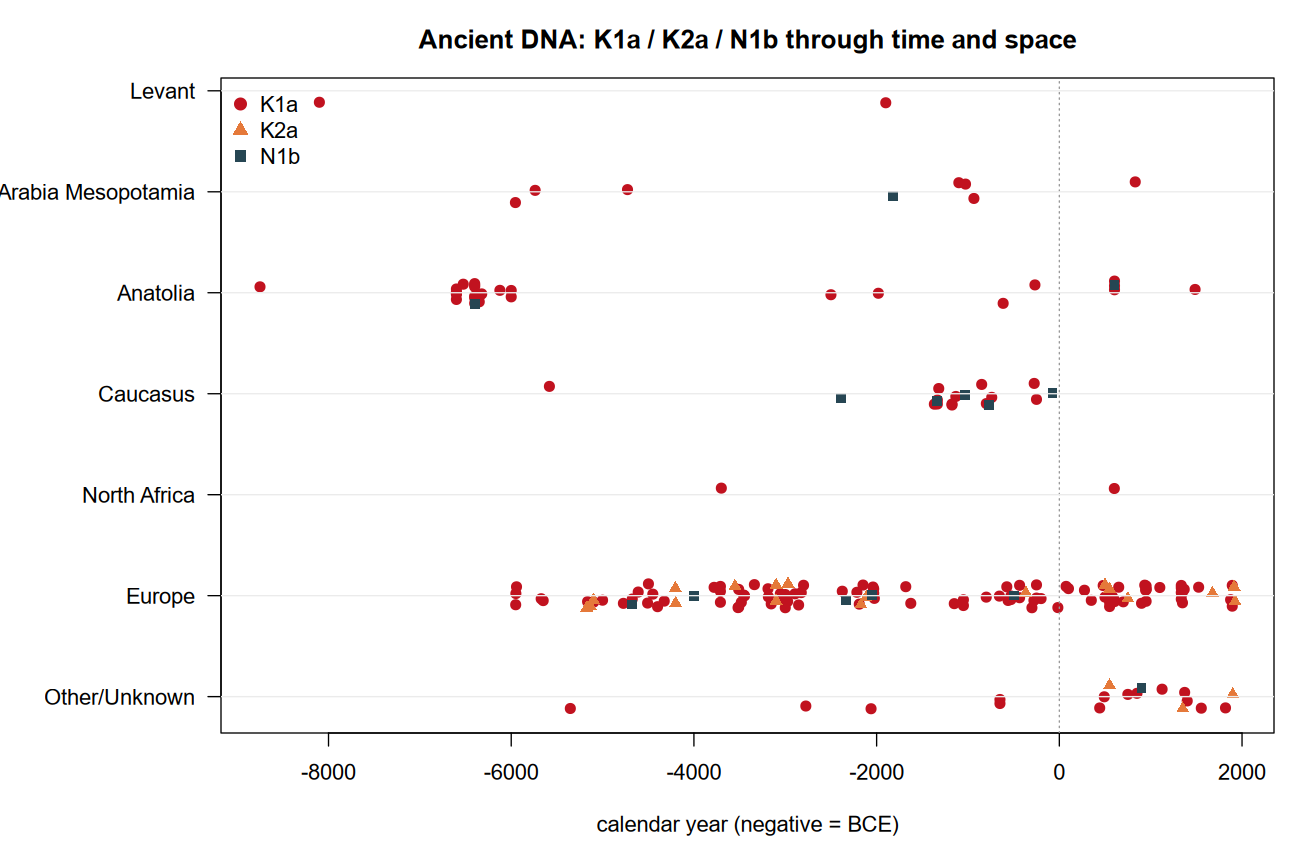
\includegraphics[width=0.82\linewidth]{../outputs/figures/C1_ancient_timeline.png}
\caption{Ancient K1a / K2a / N1b records through time and space.}
\label{fig:c1}
\end{figure}
\begin{table}[htbp]
\centering
\small
\caption{Coalescence ages (TMRCA) of founders versus parent clades.}
\label{tab:coal}
\begin{tabular}{lllll}
\toprule
haplogroup & tmrca & tmrca\_lo & tmrca\_hi & ntips \\
\midrule
K1a & 10866 & 10689 & 11045 &  6233 \\
K1a1b & 10684 &  9442 & 12002 &  1097 \\
K1a1b1 &  7222 &  6204 &  8318 &   891 \\
K1a1b1a &  2834 &  2500 &  3189 &   562 \\
K1a9 &  2845 &  2486 &  3226 &   153 \\
K2a & 13418 & 10617 & 16543 &  1276 \\
K2a2a &  5379 &  4738 &  6059 &   198 \\
N1b & 32346 & 26500 & 38766 &   708 \\
N1b2 &  5969 &  3002 &  9938 &     8 \\
\bottomrule
\end{tabular}
\end{table}
\begin{figure}[htbp]
\centering
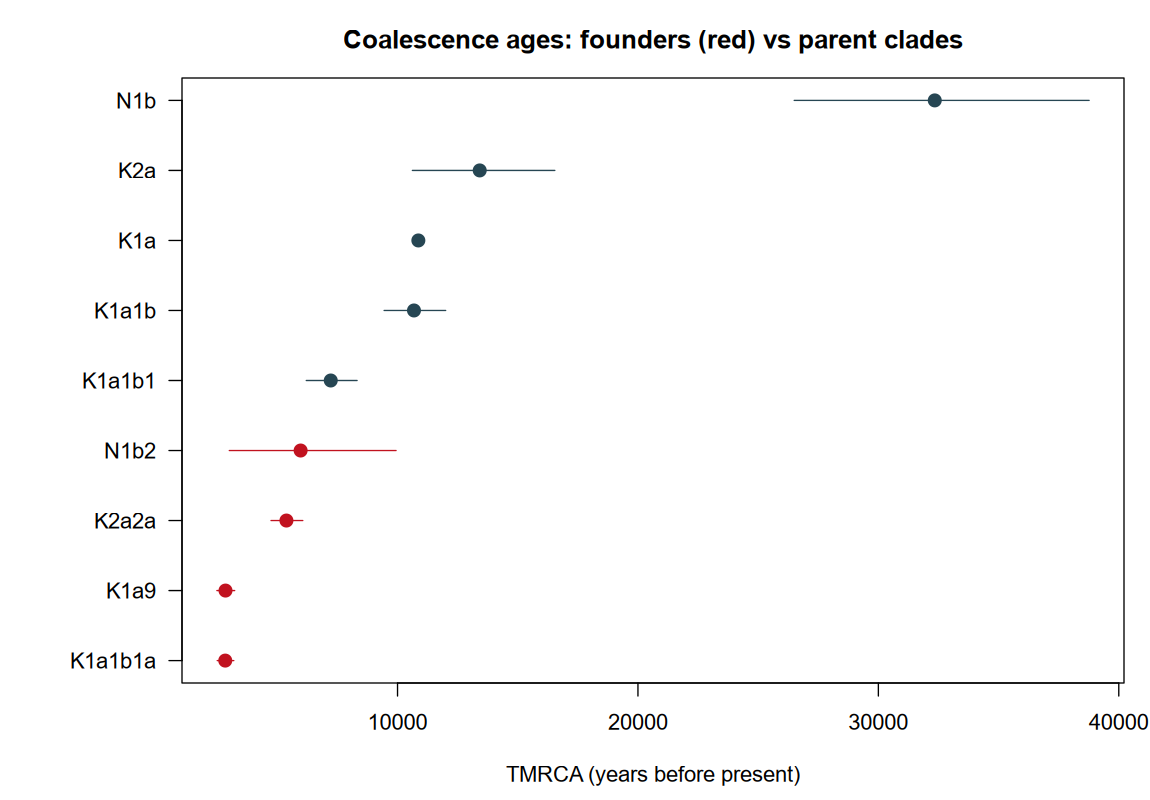
\includegraphics[width=0.82\linewidth]{../outputs/figures/C2_coalescence_ages.png}
\caption{TMRCA of founders (recent) versus their much older parent clades.}
\label{fig:c2}
\end{figure}
\begin{figure}[htbp]
\centering
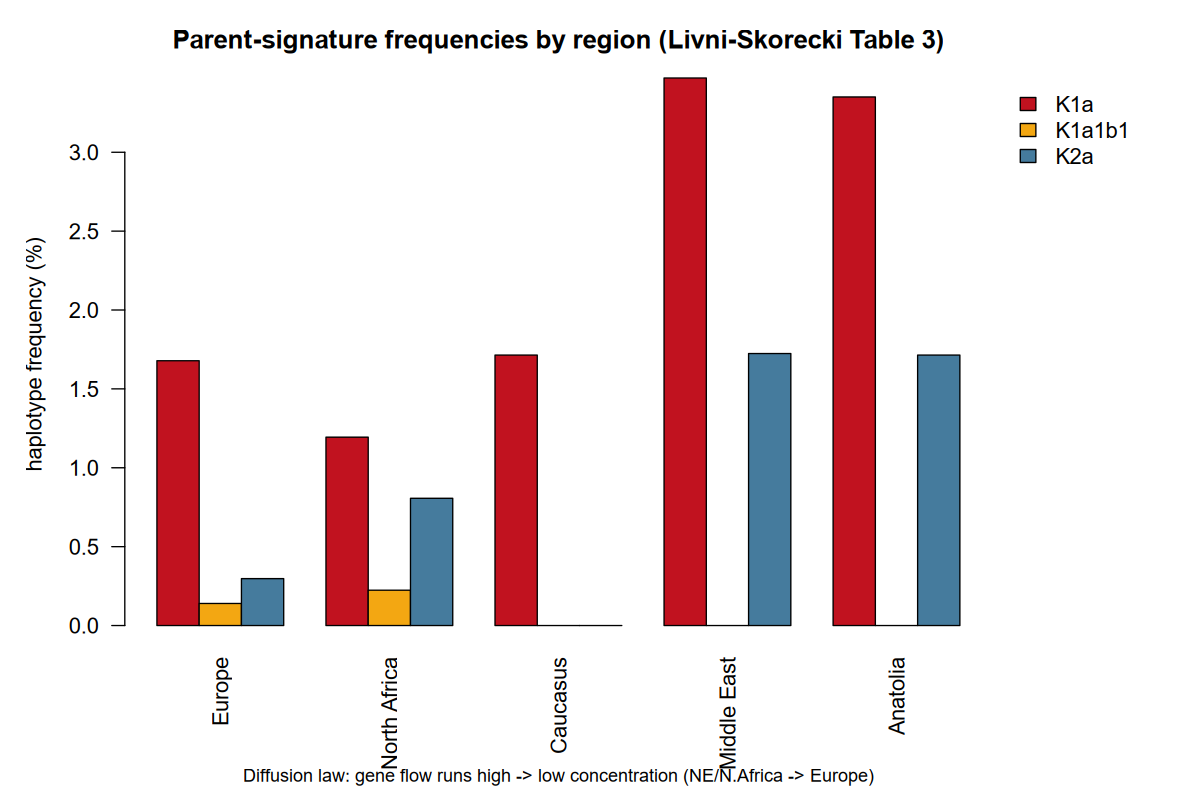
\includegraphics[width=0.82\linewidth]{../outputs/figures/C3_diffusion_frequencies.png}
\caption{Parent-signature frequencies by region (diffusion-law context).}
\label{fig:c3}
\end{figure}
Regional parent-signature frequencies for the founder macro-clades are summarized in Figure~\ref{fig:c3}. We also apply the same regional-frequency-gradient display to control clades (Figure~\ref{fig:c3b}). European-assigned controls (H, U5, J1c) peak in Europe or are Europe-rich; Near Eastern-assigned controls (R0a, U7, U1) peak in Middle East, Caucasus or Anatolia in this Mitotree/GenBank reference set. H6a1a is shown separately as the Mitotree-supported parent/context for the disputed Ashkenazi H6a1a1a lineage, not as a clean published-European control. This supports using Table 3 as directional context while keeping it a supporting benchmark rather than a stand-alone origin proof.

\begin{figure}[htbp]
\centering
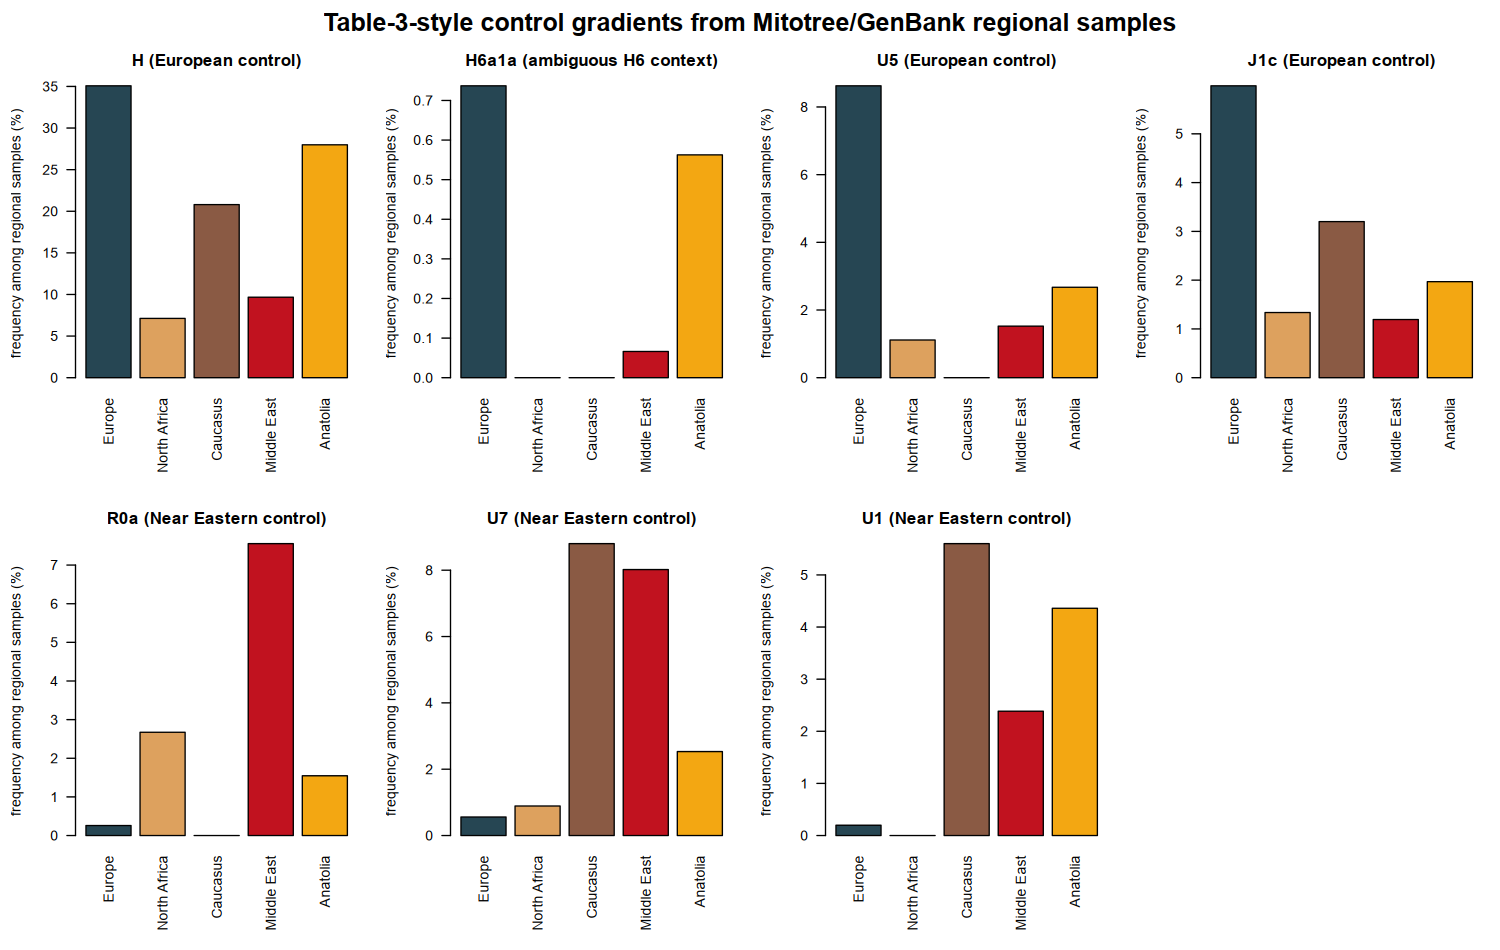
\includegraphics[width=0.82\linewidth]{../outputs/figures/C3b_table3_controls.png}
\caption{Table-3-style frequency-gradient controls from Mitotree/GenBank regional samples: European controls (H, U5, J1c), Near Eastern controls (R0a, U7, U1), and H6a1a as ambiguous H6 context.}
\label{fig:c3b}
\end{figure}
\subsection{Medieval Jewish anchors}
Founder clades appear directly in medieval Jewish individuals. In Erfurt (14th century), 11 of 31 unrelated individuals carried K1a1b1a, with additional K1a9 and N1b2/N1b1b1 carriers. In the Tarrega Roquetes pogrom sample (1348; Pallares-Vina et al., 2026), individual ROQ12 is K1a1b1a. These records move the argument from modern-frequency inference to demonstrated medieval Jewish presence. (The Erfurt K1a9 and N1b1b1 individuals come from the AADR compilation used in the stress tests, not from the Mitotree ancient subset tabulated in Table~\ref{tab:anc}.)

An independent and earlier anchor comes from Norwich, England: Brace et al. (2022) sequenced six individuals from a medieval well (radiocarbon 1161--1216 calCE, consistent with the historically attested antisemitic massacre of 1190 CE) and found strong genetic affinity to modern Ashkenazi Jews (a qpAdm model of 100\% Chapelfield fits present-day Ashkenazim), together with Ashkenazi-associated disease alleles already near modern frequency. Three of the Norwich individuals carried mitochondrial haplogroup H5c2, of which Ashkenazi Jews are the majority of modern carriers. Norwich does not sample the four K/N founders directly, but it independently demonstrates that a distinctively Ashkenazi maternal pool -- and the founder event that shaped it -- pre-dates the 12th century, corroborating the deep continuity that the founder hypothesis requires.

A nomenclature note: the Ashkenazi founder here labelled N1b2 (following Behar and Costa) is resolved as N1b1b1 on Family Tree DNA's February 2025 mitochondrial tree and in Brook (2022); 23andMe still reports it as N1b2, and the true PhyloTree N1b2 is essentially absent from Ashkenazim. The medieval Erfurt carrier belongs to this N1b1b1 clade. We retain the widely used N1b2 label for continuity with the prior literature.

\begin{table}[htbp]
\centering
\footnotesize
\caption{Ancient / historical founder-clade records in the enriched dataset.}
\label{tab:anc}
\begin{tabular}{llllll}
\toprule
Founder & Subject & Haplogroup & Country & Year & Study \\
\midrule
K1a1b1a & I13862 & K1a1b1a+16223 & Germany &  1335 & Waldman 2022 \\
K1a1b1a & I13866 & K1a1b1a+16223 & Germany &  1335 & Waldman 2022 \\
K1a1b1a & I13870 & K1a1b1a & Germany &  1335 & Waldman 2022 \\
K1a1b1a & I14846 & K1a1b1a+16223 & Germany &  1335 & Waldman 2022 \\
K1a1b1a & I14741 & K1a1b1a+16223 & Germany &  1341 & Waldman 2022 \\
K1a1b1a & Genes2026\_ROQ12 & K1a1b1a & Spain &  1348 & Pallares-Vina 2026 \\
K1a1b1a & Sobibor3 & K1a1b1a+16223 & Poland &  1893 & Diepenbroek 2021 \\
K1a1b1a & Sobibor5 & K1a1b1a+16223 & Poland &  1893 & Diepenbroek 2021 \\
K1a9 & I34375 & K1a9 &  &  1554 & Akbari 2026 \\
K2a2a & Human\_Tsavo\_H4 & K2a2a1 & Kenya &  1898 & de Flamingh 2024 \\
K2a2a & Sobibor9 & K2a2a1 & Poland &  1913 & Diepenbroek 2021 \\
K2a2a & Sobibor4 & K2a2a1 & Poland &  1923 & Diepenbroek 2021 \\
\bottomrule
\end{tabular}
\end{table}
\section{Discussion}
The five analyses assembled here point consistently in one direction. Each attacks the problem differently -- a branching-process treatment of lineage survival, a sampling-controlled test of the nesting argument, an ancient-DNA record, a non-Jewish rarity benchmark, and a Bayesian synthesis -- yet none supports a European origin for any of the four founders, and every one either favors or is consistent with a Near Eastern origin; N1b2 is the most tentative, its Europe-leaning equal-$n$ nesting tempering an otherwise Near Eastern signal, but it too stays above parity. K2a2a rests on the narrowest evidential base: once its own carriers are excluded there is a single Near Eastern sister sample within K2a, so its nesting is measured at K and near parity, and its score comes mainly from rarity and medieval Jewish carriers. The convergence of methodologically independent lines of evidence is itself the central result: it is difficult to construct a European-assimilation scenario that simultaneously reproduces the founder-tail position of all four lineages, their near-total absence among non-Jews, the equal-sample-size nesting, the deep Neolithic Near Eastern K frequency, and the medieval Jewish carriers. A further, orthogonal observation points the same way: the Ashkenazi maternal pool also carries lineages of deep African or Asian origin (notably L2a1l2a, about 2.2\%, already present at Erfurt), which a purely European source could not have supplied and which instead reflect the cosmopolitan diaspora history of a Near Eastern / Mediterranean Jewish population.



The branching model underpins this interpretation. Under realistic reproduction -- Poisson, geometric, or any intermediate negative-binomial law, and under piecewise historical growth as well as constant growth -- a lineage that survived the founder bottleneck and rose to the observed frequencies is overwhelmingly likely to appear in many copies, whereas a recently absorbed host matriline appears as a singleton. The measured absorbed fraction ($a_\epsilon \approx 0.22$ in the largest available sample) confirms that the four major founders sit in the founder tail, not the host tail. Consistent with this, the Euro-Levantine reconciliation -- in which a large Roman-era population generates three or more of the founders by private mutation -- carries only a 1.51\% probability.

Genome-wide studies frame and, on balance, reinforce a Near Eastern origin for the Jewish autosomal core. Atzmon et al. (2010) showed that the major Jewish Diaspora groups form distinct clusters with shared Middle Eastern ancestry, and framed the four mtDNA founders (about 40\% of the Ashkenazi maternal pool) as Middle Eastern in origin. Agranat-Tamir et al. (2020) supply the deep ancient-DNA anchor: Bronze Age 'Canaanite' genomes of the Southern Levant to which present-day Jewish groups, including Ashkenazi Jews, trace 50\% or more of their ancestry. Carmi et al. (2014) document the severe late-medieval bottleneck and roughly even European / Middle Eastern autosomal ancestry.

The complementary European component is real and well characterised, but it is predominantly Southern European and does not bear directly on the maternal founders. Xue et al. (2017) date this gene flow to at least two events around the founder bottleneck, and recent local-ancestry inference (Lerga-Jaso et al., 2025) assigns Ashkenazi Jews a large Italian / Southern European component alongside a Levantine one. Because Southern European populations themselves carry substantial Near Eastern ancestry, and because autosomal ancestry is not uniparental, a large Southern European autosomal fraction is fully compatible with --- and indeed expected under --- a Levantine maternal core (H2) followed by later European admixture; it does not imply that the maternal founders were European.

Two caveats bound but do not overturn the conclusion. First, the Pre-Pottery Neolithic K samples (Fernandez et al., 2014) were typed only on the control region and cannot be resolved to the specific K1a1b1a or K2a2a sub-motifs; they establish deep Near Eastern K at the macro-clade level rather than the founder sub-clade level. Second, lineage loss through drift means the absence of a derived sub-clade in a small ancient panel is not proof of its past absence. Both caveats limit the resolution of the ancient-DNA channel. They weaken over-specific claims at the founder-subclade level, but they do not supply positive evidence for the recent European-host origin model.

\section{Conclusions}
Integrating a branching-process model, a phylogeographic rarefaction analysis, an ancient-DNA record, a non-Jewish rarity benchmark, and a ridge-logistic origin synthesis over the largest available maternal reference dataset, we find that all four major Ashkenazi mtDNA founders -- K1a1b1a, K1a9, K2a2a and N1b2 -- are best explained by a Near Eastern / Levantine origin. The support is strongest for the two K1a founders (K1a9 0.994, K1a1b1a 0.988, credible intervals excluding parity), then K2a2a (0.899), and is positive though most tentative for N1b2 (0.891), whose Europe-leaning nesting tempers its rarity and antiquity signals. No founder is better explained by a simple prehistoric European-host origin under the analyses performed here.

These results support and extend the Livni--Skorecki (2025) and Behar et al. (2006) Near Eastern model relative to the Costa et al. (2013) European-assimilation model, and they do so with an explicit, reproducible quantification of the uncertainty. Mitochondrial DNA alone cannot fix a geographic origin with the precision of genome-wide data, and finer resolution -- coding-region typing of ancient Near Eastern K and N carriers, and dense Levantine population sampling -- would sharpen the N1b2 estimate in particular. On present evidence, however, the Near Eastern origin of the Ashkenazi maternal founder core is the parsimonious and best-supported conclusion.

\vspace{0.5em}
\noindent\textit{Reproducibility.} All results, tables, and figures are reproduced end-to-end from the public Mitotree release, GenBank queries, and the cited study data by a single analysis script.
\section{Limitations}
\begin{itemize}
\item \textbf{Reference-set sampling.} Mitotree/GenBank is a cross-study reference set; we treat it as the largest available maternal sample and estimate absorption from its singleton fraction, but that fraction is sensitive to lineage-calling resolution and global (non-Ashkenazi) diversity, so the enriched-set estimate is an upper bound and Behar 2006 is the Ashkenazi-specific anchor.
\item \textbf{Diaspora bias.} Modern country reflects residence, not origin, and is not used as direct evidence of origin.
\item \textbf{Public subset.} The public Mitotree release is a subset of the full phylogeny; ancient Near Eastern coverage is sparse.
\item \textbf{YFull/FTDNA public enrichment.} Public genealogy pages improve alias resolution, branch-age context and ancient-anchor visibility, but tester country/project counts are participation-biased and are not treated as population frequencies.
\item \textbf{Literature-coded controls.} Some non-founder controls use published classifications and manually curated frequencies rather than being discovered de novo from Mitotree. They are used for calibration and falsification, not as independent population estimates.
\item \textbf{Regularized logistic synthesis.} Channel weights are fit to a small labeled panel with ridge priors and leave-one-out validation; the posterior is an evidence synthesis, not a fully generative demographic likelihood. European controls (V7, U5) use 1000 Genomes EUR (n=503) subclade frequencies and score far below all four founders.
\item \textbf{Branching independence.} The Galton--Watson layer assumes independent offspring counts conditional on the chosen law and generation. Negative-binomial overdispersion and piecewise growth test sensitivity to realistic variance and timing, but they do not model full family-level correlation or overlapping generations.
\item \textbf{Reconstructed motifs.} The haplotype network and glPCA use motifs reconstructed from Mitotree defining-mutation strings, not per-sample alignments.
\item \textbf{Model framework.} The branching equations are used both as a sensitivity framework and, via the singleton fraction, as an absorption-rate estimator; the estimate is a moment-style estimate, not a full likelihood fit with per-individual sampling weights.
\item \textbf{Not a primary study.} This pipeline integrates public data to test H2 against H1; it is not a substitute for peer-reviewed primary analysis.
\end{itemize}
\appendix
\section{Computational Appendix: Core Algorithm Excerpts}
\label{app:code}
The full source code is the reproducible record. The excerpts below are included because they define the computational genetics operations most likely to affect interpretation: tree traversal, branching-process coefficient recovery, rarefaction, public-page time adjustment, and Bayesian score construction. Boilerplate plotting, file I/O and table formatting are intentionally omitted.

\subsection{Mitotree descendant traversal}
All clade counts use graph traversal over the Mitotree parent-child table. A sample is inside a clade if its resolved haplogroup is a member of the descendant set.

\begingroup\footnotesize
\begin{verbatim}
build_topology <- function(struct) {
  parent <- setNames(struct$ParentHaplogroup, struct$Haplogroup)
  children <- split(struct$Haplogroup, struct$ParentHaplogroup)
  list(parent = parent, children = children, nodes = struct$Haplogroup)
}

descendants <- function(root, topo, include_self = TRUE) {
  out <- character(0); stack <- root
  while (length(stack)) {
    node <- stack[[1]]; stack <- stack[-1]
    if (node %in% out) next
    out <- c(out, node)
    stack <- c(stack, topo$children[[node]])
  }
  if (!include_self) setdiff(out, root) else out
}
\end{verbatim}
\endgroup
\subsection{Branching-process PGF composition}
The descendant-count distribution after $k$ generations is recovered by composing offspring probability-generating functions and inverting the coefficients by FFT. This avoids slow repeated convolutions while preserving an audit path: the paper also writes a direct-convolution check to \texttt{A\_branching\_math\_audit.csv}.

\begingroup\footnotesize
\begin{verbatim}
gw_descendant_pmf <- function(m, k = GW_K, jmax = NULL, model, size = 1) {
  if (length(m) == 1L) m <- rep(m, k)
  # The inverse FFT ALIASES mass above the grid back onto low j rather than
  # truncating it, so the grid is sized from E[Z_k] = prod(m).
  N <- if (is.null(jmax)) 2^ceiling(log2(max(512, 64 + 40 * prod(m)))) else jmax + 1L
  omega <- exp(-2i * pi * (0:(N - 1)) / N)
  eval_pgf <- function(z, off) {
    val <- complex(length(z))
    for (jj in seq(length(off) - 1, 0)) val <- val * z + off[jj + 1]
    val
  }
  gz <- omega
  for (t in rev(seq_len(k))) {
    off <- gw_offspring_pmf(m[t], jmax = jmax, model = model, size = size)
    gz <- eval_pgf(gz, off)
  }
  p <- Re(fft(gz, inverse = TRUE) / N)
  p[p < 0] <- 0; p / sum(p)
}
\end{verbatim}
\endgroup
\subsection{Rarefied nesting score}
The Costa nesting claim is evaluated after equalizing sample size. The model uses expected sub-lineage richness at matched $n$, not raw European and Near Eastern counts.

\begingroup\footnotesize
\begin{verbatim}
# .rarefy_at_root() in R/lineage_data.R; sketch:
rarefy_at_root <- function(root) {
  s <- B_rar[B_rar$root == root, ]
  nmax <- max(s$n[!is.na(s$distinct_lineages)])
  w <- s[s$n == nmax, ]
  list(ne = w$distinct_lineages[w$region == 'Near East'],
       eu = w$distinct_lineages[w$region == 'Europe'],
       ne_pool = s$pool_size[s$region == 'Near East'][1],
       eu_pool = s$pool_size[s$region == 'Europe'][1])
}

# positive = Near East (or non-Europe) richer at equal n; a single z_nest
# weight is fit across all lineages, so the sign is NOT flipped by macro-clade.
s_nest <- (ne_richness - eu_richness) / (ne_richness + eu_richness)
# richness is DEPTH-MATCHED, and s_nest is then shrunk toward 0 by its own
# bootstrap SE:  s_nest * s_nest^2 / (s_nest^2 + se^2)
\end{verbatim}
\endgroup
\subsection{Origin synthesis (standardized channels + ridge logistic)}
Raw channels are z-scored across scored lineages; a ridge-logistic model is fit to labeled controls with founders held out. Coefficient uncertainty is propagated by Laplace-approximation Monte Carlo.

\begingroup\footnotesize
\begin{verbatim}
z <- function(x) (x - mean(x, na.rm = TRUE)) / sd(x, na.rm = TRUE)
X <- cbind(1, z_freq, z_time, z_nest)
fit <- fit_logistic_bayes(train)   # ridge priors tau = 2, tau0 = 5
draws <- fit$draws                 # M = 40000 Laplace-approximation draws
p <- plogis(X %*% t(draws))
\end{verbatim}
\endgroup
\subsection{Public YFull/FTDNA time adjustment}
Public genealogy data enter only through bounded branch-age and ancient-anchor context. Tester country/project counts remain descriptive and do not enter the frequency channel.

\begingroup\footnotesize
\begin{verbatim}
public_time_adjustment <- function(tmrca_kyr, confidence, ancient_anchor,
                                   medieval_carriers) {
  if (is.na(tmrca_kyr) || confidence <= 0) return(0)
  recent_penalty <- if (tmrca_kyr < 1) -0.25 * confidence else 0
  # carriers are their own sub-channel of z_time, so they must NOT also
  # set `anchored` here -- that would count one record twice in one channel.
  anchored <- public_jewish_ancient_anchor > 0
  mature_bonus <- if (anchored && tmrca_kyr >= 1.5) 0.12 * confidence else 0
  recent_penalty + mature_bonus
}
\end{verbatim}
\endgroup
\section*{References}
\begin{itemize}\small
\item Livni J. \& Skorecki K. (2025) Distinguishing between founder and host population mtDNA lineages in the Ashkenazi population. Human Gene; SSRN 5035272.
\item Costa M.D. et al. (2013) A substantial prehistoric European ancestry amongst Ashkenazi maternal lineages. Nat. Commun. 4:2543.
\item Behar D.M. et al. (2006) The matrilineal ancestry of Ashkenazi Jewry. Am. J. Hum. Genet. 78:487--497.
\item Atzmon G. et al. (2010) Abraham's children in the genome era: major Jewish Diaspora populations comprise distinct genetic clusters with shared Middle Eastern ancestry. Am. J. Hum. Genet. 86:850--859.
\item Carmi S. et al. (2014) Sequencing an Ashkenazi reference panel supports population-targeted personal genomics and illuminates Jewish and European origins. Nat. Commun. 5:4835.
\item Agranat-Tamir L. et al. (2020) The genomic history of the Bronze Age Southern Levant. Cell 181:1146--1157.
\item Lerga-Jaso J. et al. (2025) Tracing human genetic histories and natural selection with precise local ancestry inference. Nat. Commun. 16:4576.
\item Xue J. et al. (2017) The time and place of European admixture in Ashkenazi Jewish history. PLoS Genet. 13(4):e1006644.
\item Waldman S. et al. (2022) Genome-wide data from medieval German Jews show that the Ashkenazi founder event pre-dated the 14th century. Cell 185:4703--4716.
\item Brace S. et al. (2022) Genomes from a medieval mass burial show Ashkenazi-associated hereditary diseases pre-date the 12th century. Curr. Biol. 32:4350--4359.
\item Fernandez E. et al. (2014) Ancient DNA analysis of 8000 B.C. Near Eastern farmers. PLoS Genet. 10(6):e1004401.
\item Shamoon-Pour M., Li M. \& Merriwether D.A. (2019) Rare human mitochondrial HV lineages spread from the Near East and Caucasus during post-LGM and Neolithic expansions. Sci. Rep. 9:14751.
\item Pallares-Vina L. et al. (2026) Uncovering a medieval pogrom: genetic history of a Jewish community in Catalonia (Spain). Genes 17(3):358.
\item Maier P.A. et al. (2026) Mitotree: the universal human mitochondrial reference phylogeny. bioRxiv.
\item 1000 Genomes Project Consortium (2015) A global reference for human genetic variation. Nature 526:68--74.
\item Diroma M.A. et al. (2014) Extraction and annotation of human mitochondrial genomes from 1000 Genomes Whole Exome Sequencing data. BMC Genomics 15(Suppl 3):S2.
\item Mitchell S.L. et al. (2014) Characterization of mitochondrial haplogroups in a large population-based sample from the United States. Hum. Genet. 133:861--868.
\item Brook K.A. (2022) The Maternal Genetic Lineages of Ashkenazic Jews. Academic Studies Press.
\item Penninx W. (2019) Analysis of mtDNA haplogroup frequencies in the Ashkenazi Jewish population (compiled in Brook 2022).
\item Wexler J.D. (2019--2026) Ashkenazi Y-DNA and mtDNA (compilation). \url{https://sites.google.com/view/ashkenazi-y-dna-and-mtdna}
\item YFull MTree (accessed by public haplogroup pages, 2026). \url{https://www.yfull.com/mtree/}
\item FamilyTreeDNA Discover public mtDNA haplogroup pages and JSON resources (accessed 2026). \url{https://discover.familytreedna.com/mtdna/}
\item FamilyTreeDNA Discover, mtDNA haplogroup V7a12a1 age estimate. \url{https://discover.familytreedna.com/mtdna/V7a12a1/classic}
\end{itemize}
\end{document}
